\documentclass[11pt,a4paper]{article}
\usepackage[utf8]{inputenc}
\usepackage[french]{babel}
\usepackage[T1]{fontenc}

\usepackage{amsmath}
\usepackage{amsfonts}
\usepackage{amssymb}

\newcommand{\TitreMatiere}{Algorithmique 1}
\newcommand{\TitreSeance}{Tris}
\newcommand{\SousTitreSeance}{Bulles, Sélection, Insertion}
\newcommand{\DateCours}{Novembre 2024}
\newcommand{\AnneeScolaire}{2024-2025}
\newcommand{\Organisation}{EPITA}
\newcommand{\NomAuteurA}{Fabrice BOISSIER}
\newcommand{\MailAuteurA}{fabrice.boissier@epita.fr}
\newcommand{\NomAuteurB}{ }
\newcommand{\MailAuteurB}{ }
\newcommand{\DocKeywords}{Algorithmique ; Algorithmes ; Tris ; Tri ; Sort ; Tri à Bulles ; Bubble Sort ; Tri par Sélection ; Selection Sort ; Tri par Insertion ; Insertion Sort}
\newcommand{\DocLangue}{fr} % "en", "fr", ...

\usepackage{MetalCourseBooklet}

% Babel ne traduit pas toujours bien les tableaux et autres
\renewcommand*\frenchfigurename{%
    {\scshape Figure}%
}
\renewcommand*\frenchtablename{%
    {\scshape Tableau}%
}

% Ne pas afficher le numéro de la légende sur tableaux et figures
\captionsetup{format=sanslabel}


\begin{document}

\EncadreTitre

\bigskip


%\begin{center}
%\begin{tabular}{p{5cm} p{11cm}}
%\textbf{Commandes étudiées :} & \texttt{sh}, \texttt{bash}, \texttt{man}, \texttt{ls}, \texttt{mkdir}, \texttt{touch}, \texttt{chmod}, \texttt{mv}, \texttt{rm}, \texttt{rmdir}, \texttt{cat}, \texttt{file}, \texttt{which}, \texttt{which}\\
%
%\textbf{Builtins étudiées :} & \texttt{pwd}, \texttt{cd}, \texttt{exit}, \texttt{logout}, \texttt{echo}, \texttt{umask}, \texttt{type}, \texttt{>}, \texttt{>{}>}, \texttt{<}, \texttt{<{}<}, \texttt{|}\\
%
%\textbf{Notions étudiées :} & Shell, Manuels, Fichiers, Répertoires, Droits, Redirections\\
%\end{tabular}
%\end{center}

\bigskip


Ce document a pour objectif de vous familiariser avec quelques algorithmes de tri afin de mieux comprendre les raisons impliquant l'existence de nombreuses méthodes de tri.


\bigskip

%%%%%%%%%%%%%%%%%%%%%%%%%%%%%%%%%%%%%%

\section{Définitions}

Définition informelle d'un algorithme de tri~\footnote{Wikipedia (octobre 2023) : \href{https://fr.wikipedia.org/wiki/Algorithme_de_tri}{Algorithme de tri}} : \og \textit{Un algorithme de tri est, en informatique ou en mathématiques, un algorithme qui permet d'organiser une collection d'objets selon une relation d'ordre déterminée.} \fg .

\bigskip

En pratique cela implique d'organiser des objets comparables les uns avec les autres selon un critère.
On peut ordonner des fruits selon leur taille, leur poids, etc.
Le critère pour ordonner doit absolument disposer d'une \textit{relation d'ordre} du type \og plus grand que \fg{} ou \og inférieur ou égal à \fg{}, afin de trier les objets (c'est-à-dire leur donner un numéro d'ordre).

\bigskip

Très concrètement, les algorithmes de tri ont comme objectif de réorganiser en ordre croissant ou décroissant un tableau composé d'éléments comparables deux à deux.
Les principaux problèmes rencontrés concernent :
\begin{itemize}
\item la \textit{complexité temporelle}, c'est-à-dire le temps nécessaire pour trier (souvent associé au nombre de comparaisons et déplacements nécessaires),
\item la \textit{complexité spatiale}, c'est-à-dire l'espace nécessaire pour réorganiser le tableau (déplacement d'au plus 2 éléments à la fois, ou construction complète d'un nouveau tableau en mémoire en parallèle de l'ancien),
\item la \textit{stabilité}, c'est-à-dire que l'on conserve l'ordre des éléments considérés comme égaux dans le tableau initial (si deux pommes P1 suivie de P2 ont le même poids, on doit conserver l'ordre en sortie P1 suivie de P2 et surtout pas P2 suivie de P1 : en effet, un tri sur un autre critère que le poids a peut être été effectué préalablement, et ainsi, les pommes seront triées principalement sur leur poids, et ensuite sur chaque critère précédent).
\end{itemize}

\bigskip

Dans ce document nous étudierons trois algorithmes très simples de tri (donc pas du tout optimaux) :
\begin{enumerate}
\item le \textit{tri à bulles} (ou \textit{bubble sort} en anglais)
\item le \textit{tri par sélection} (ou \textit{selection sort} en anglais)
\item le \textit{tri par inserion} (ou \textit{insertion sort} en anglais)
\end{enumerate}
Ces algorithmes vous permettront de comprendre les différences de traitements (et donc d'états intermédiaires) pour obtenir les mêmes résultats à partir de la même entrée.

\bigskip

Les algorithmes vus dans ce document s'appuient sur des tableaux en mémoire dont la longueur est conservée dans une variable distincte (exactement comme en C).
Lorsque l'on donnera un tableau en paramètre, il faudra lui adjoindre un second paramètre qui sera la longueur exacte du tableau sous forme d'entier.

En d'autres termes, dans ce document, le tableau n'embarque pas sa taille comme c'est le cas en Python.

\bigskip

\`A noter également : on parle de \textit{tri en place} lorsqu'on ne fait que modifier le tableau donné en paramètre sans jamais créer un deuxième tableau intermédiaire.
D'ailleurs, ces algorithmes ne retournent rien, car le tableau est déjà alloué : il suffit de le modifier.


%\bigskip
\clearpage

%%%%%%%%%%%%%%%%%%%%%%%%%%%%%%%%%%%

\section{Swap}

\medskip

Avant de démarrer les tris, il est très utile d'avoir une fonction permettant d'échanger deux valeurs dans un tableau.

Cette opération très simple peut être implémentée comme ceci.
Vous noterez que le paramètre \textit{tab} est le tableau, et le paramètre \textit{len} est la longueur de ce tableau.

%\medskip

\vfillFirst

\begin{table}[ht!]
  \centering
% %*   *)
\begin{lstlisting}[style=algorithmique]
algorithme fonction SwapV1 : booleen
  parametres locaux
    entier[]  tab
    entier    len, pos1, pos2
  variables
    entier    var
debut
si (pos1 > (len - 1)) ou (pos2 > (len - 1)) alors
  retourner (faux)
sinon si (pos1 < 0) ou (pos2 < 0) alors
  retourner (faux)
sinon
  var = tab[pos1]
  tab[pos1] = tab[pos2]
  tab[pos2] = var
  retourner (vrai)
fin si
fin algorithme fonction SwapV1 \end{lstlisting}
%  \caption{Bla. }
%  \label{puissance}
\end{table}


\begin{table}[ht!]
  \centering
% %*   *)
\begin{lstlisting}[style=algorithmique]
algorithme fonction SwapV2 : booleen
  parametres locaux
    entier[]  tab
    entier    len, pos1, pos2
  variables
    entier    var
debut
si (pos1 >= 0) et (pos1 < len) et
   (pos2 >= 0) et (pos2 < len) alors
  var = tab[pos1]
  tab[pos1] = tab[pos2]
  tab[pos2] = var
  retourner (vrai)
sinon
  retourner (faux)
fin si
fin algorithme fonction SwapV2 \end{lstlisting}
%  \caption{Bla. }
%  \label{puissance}
\end{table}


\vfillLast

\clearpage
%\bigskip

%%%%%%%%%%%%%%%%%%%%%%%%%%%%%%%%%%%

\section{Tri à Bulles}

\medskip

Le tri à bulles vise à faire remonter tour à tour les plus grandes valeurs vers la fin du tableau.

\medskip

Si deux valeurs côte à côte sont dans le désordre, on les inverse, et on teste les suivantes jusqu'à la fin du tableau.
On recommence ce traitement sur chaque case du tableau autant de fois que nécessaire (c'est-à-dire autant de fois qu'il y a de cases).

\medskip

Avec cette méthode, dès que l'on trouve la plus grande valeur du tableau, celle-ci avancera progressivement jusqu'à la fin.
Avant d'atteindre la plus grande valeur, on peut également faire remonter les autres grandes valeurs.
Cependant, à chaque fois que l'on parcourt intégralement le tableau de gauche à droite, on est sûr que la valeur la plus à droite est à sa place finale.
Ainsi, on réduit la zone à parcourir à chaque tour : une fois la plus grande valeur du tableau trouvée à la fin du premier tour et placée à la dernière case, on n'a plus besoin de chercher dans cette case (l'élément étant maintenant à sa place).

\medskip

\begin{itemize}
\item Complexité moyenne : $ T(n) = O(n^{2}) $
\item Complexité pire cas : $ T(n) = O(n^{2}) $
\item Complexité meilleur cas : $ T(n) = O(n) $
\item Tri en place
\item Tri stable
\end{itemize}


\medskip


%\begin{figure*} % Figure flottante
\begin{figure}[ht!]
\centering
\centerline{
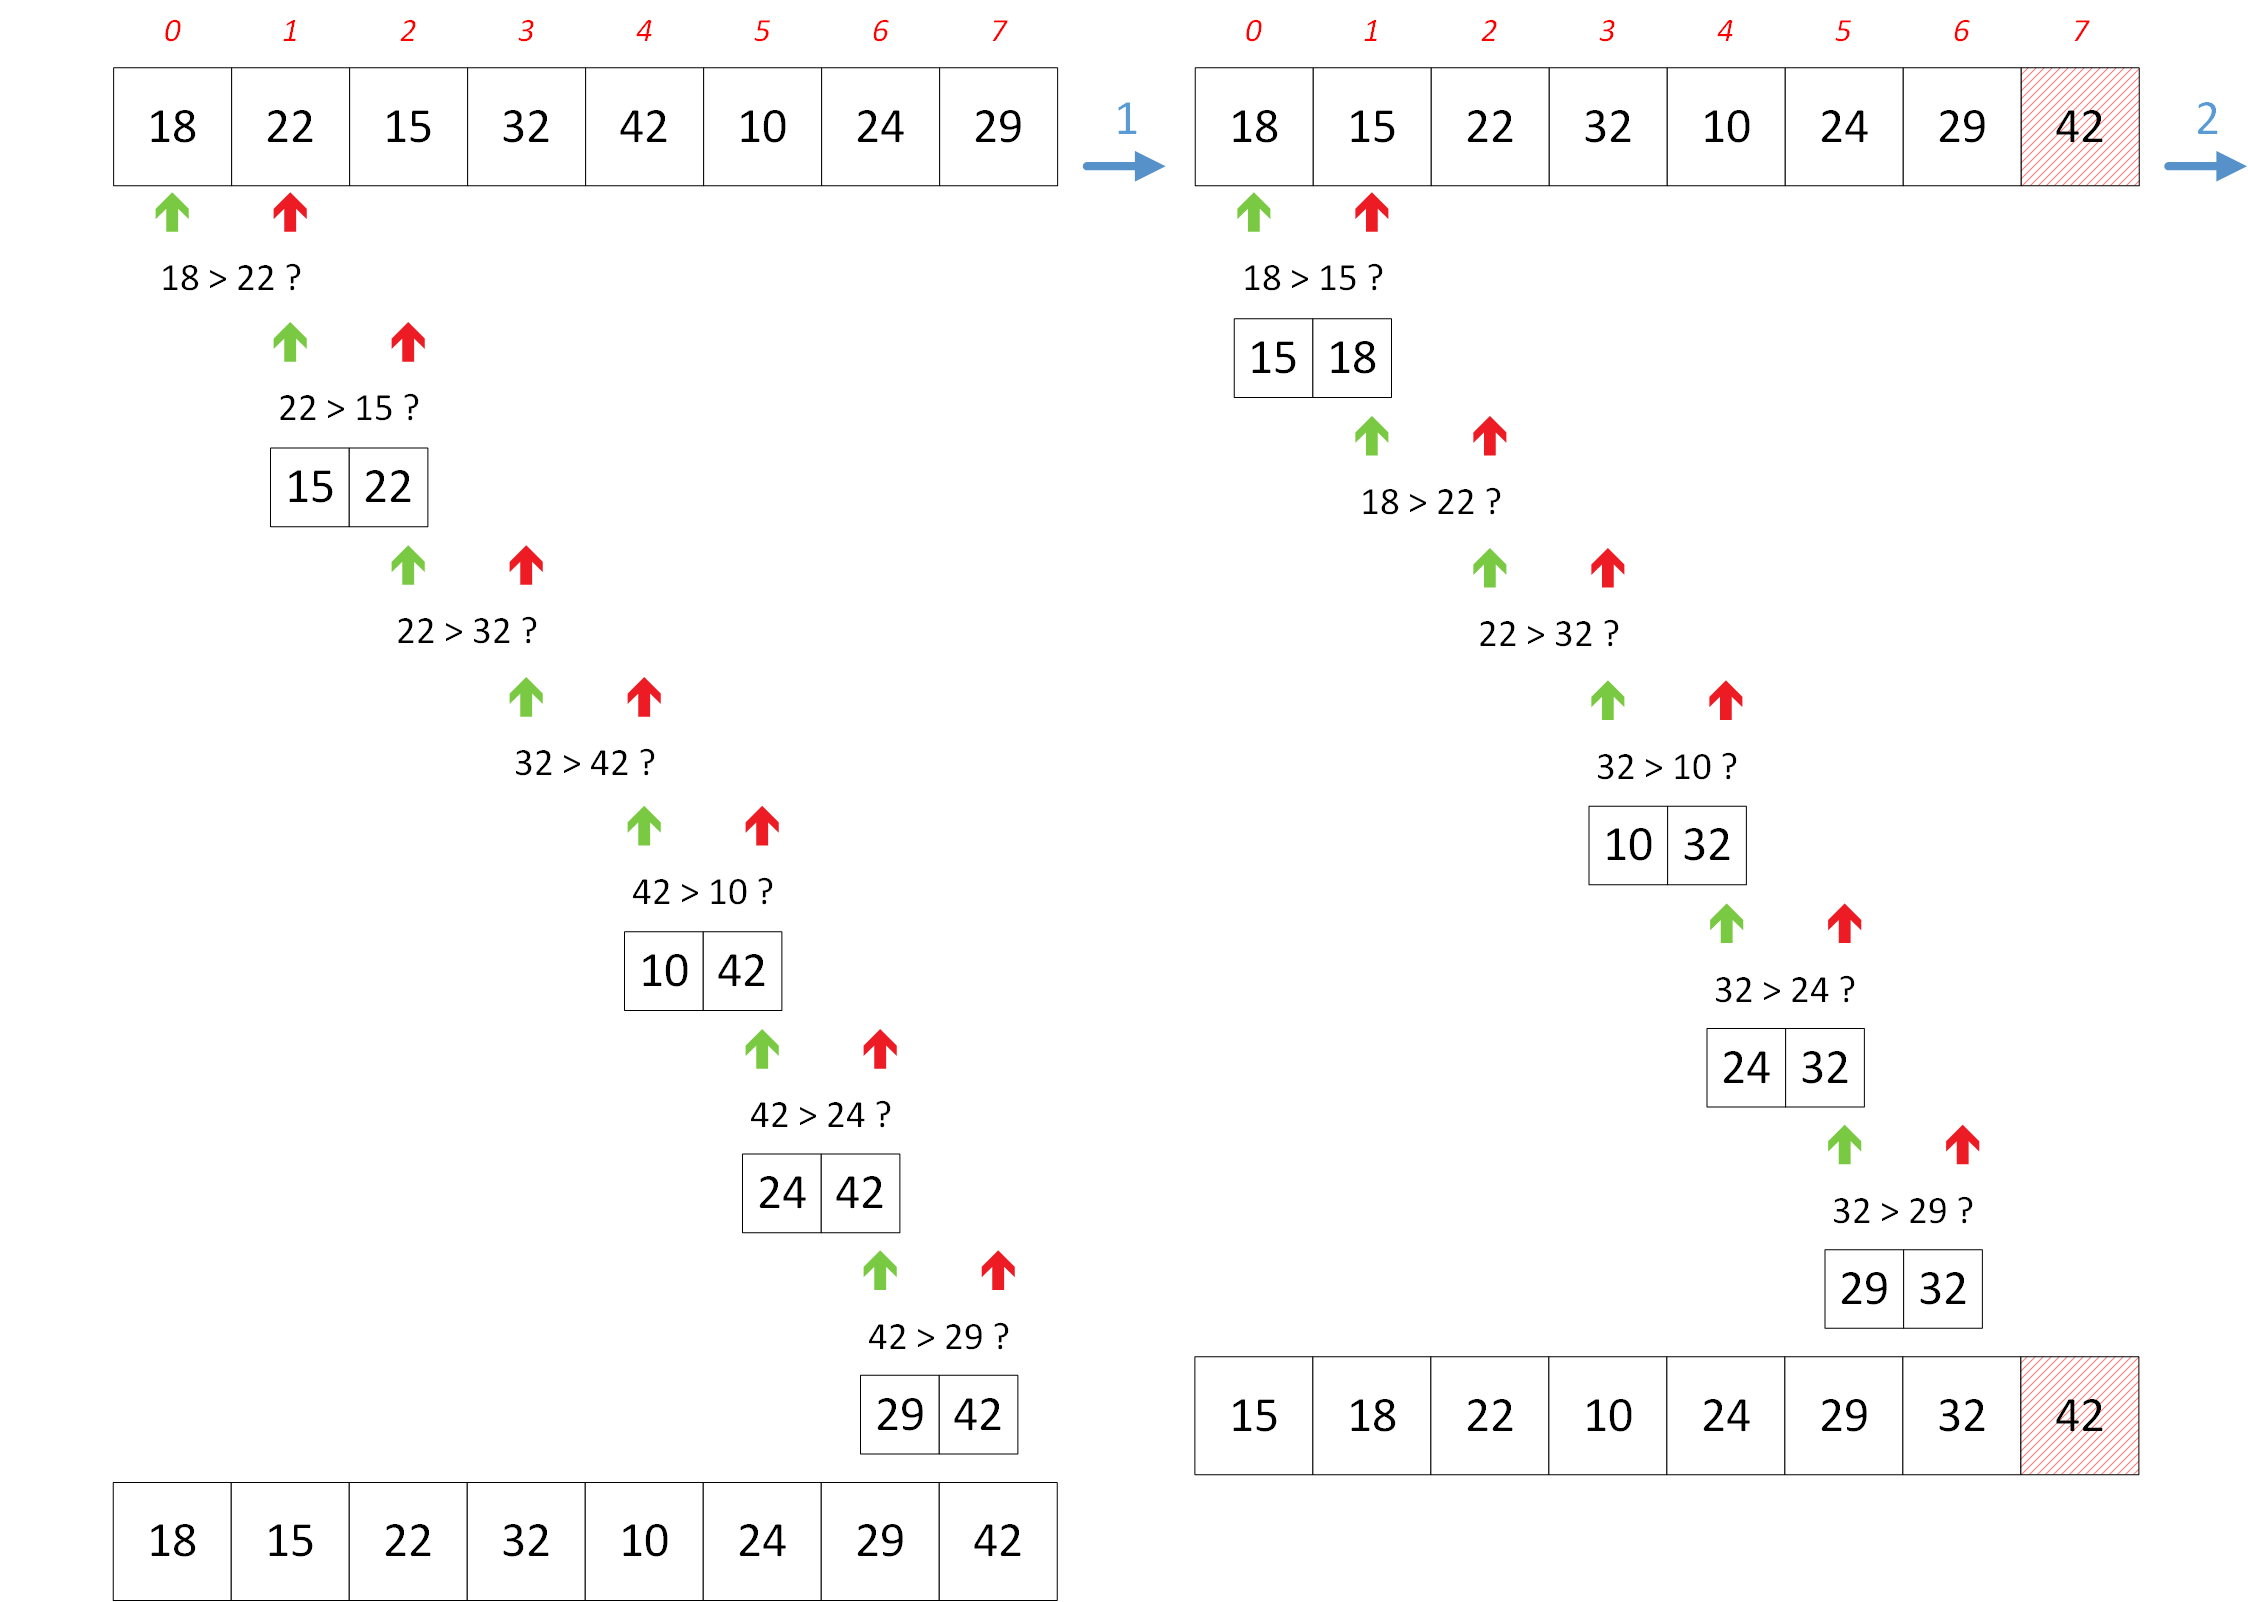
\includegraphics[width=1.2\textwidth]{img/tris/2_per_pages/BubbleSort_part1.png}
}
%\caption{Bubble Sort part 1}
%\label{figure:1-S3-DesignScience-ThreeLoops}
\end{figure}
%\end{figure*} % Figure flottante
% To use it : fig~\ref{label}

\clearpage

%\begin{figure*} % Figure flottante
\begin{figure}[ht!]
\centering
\centerline{
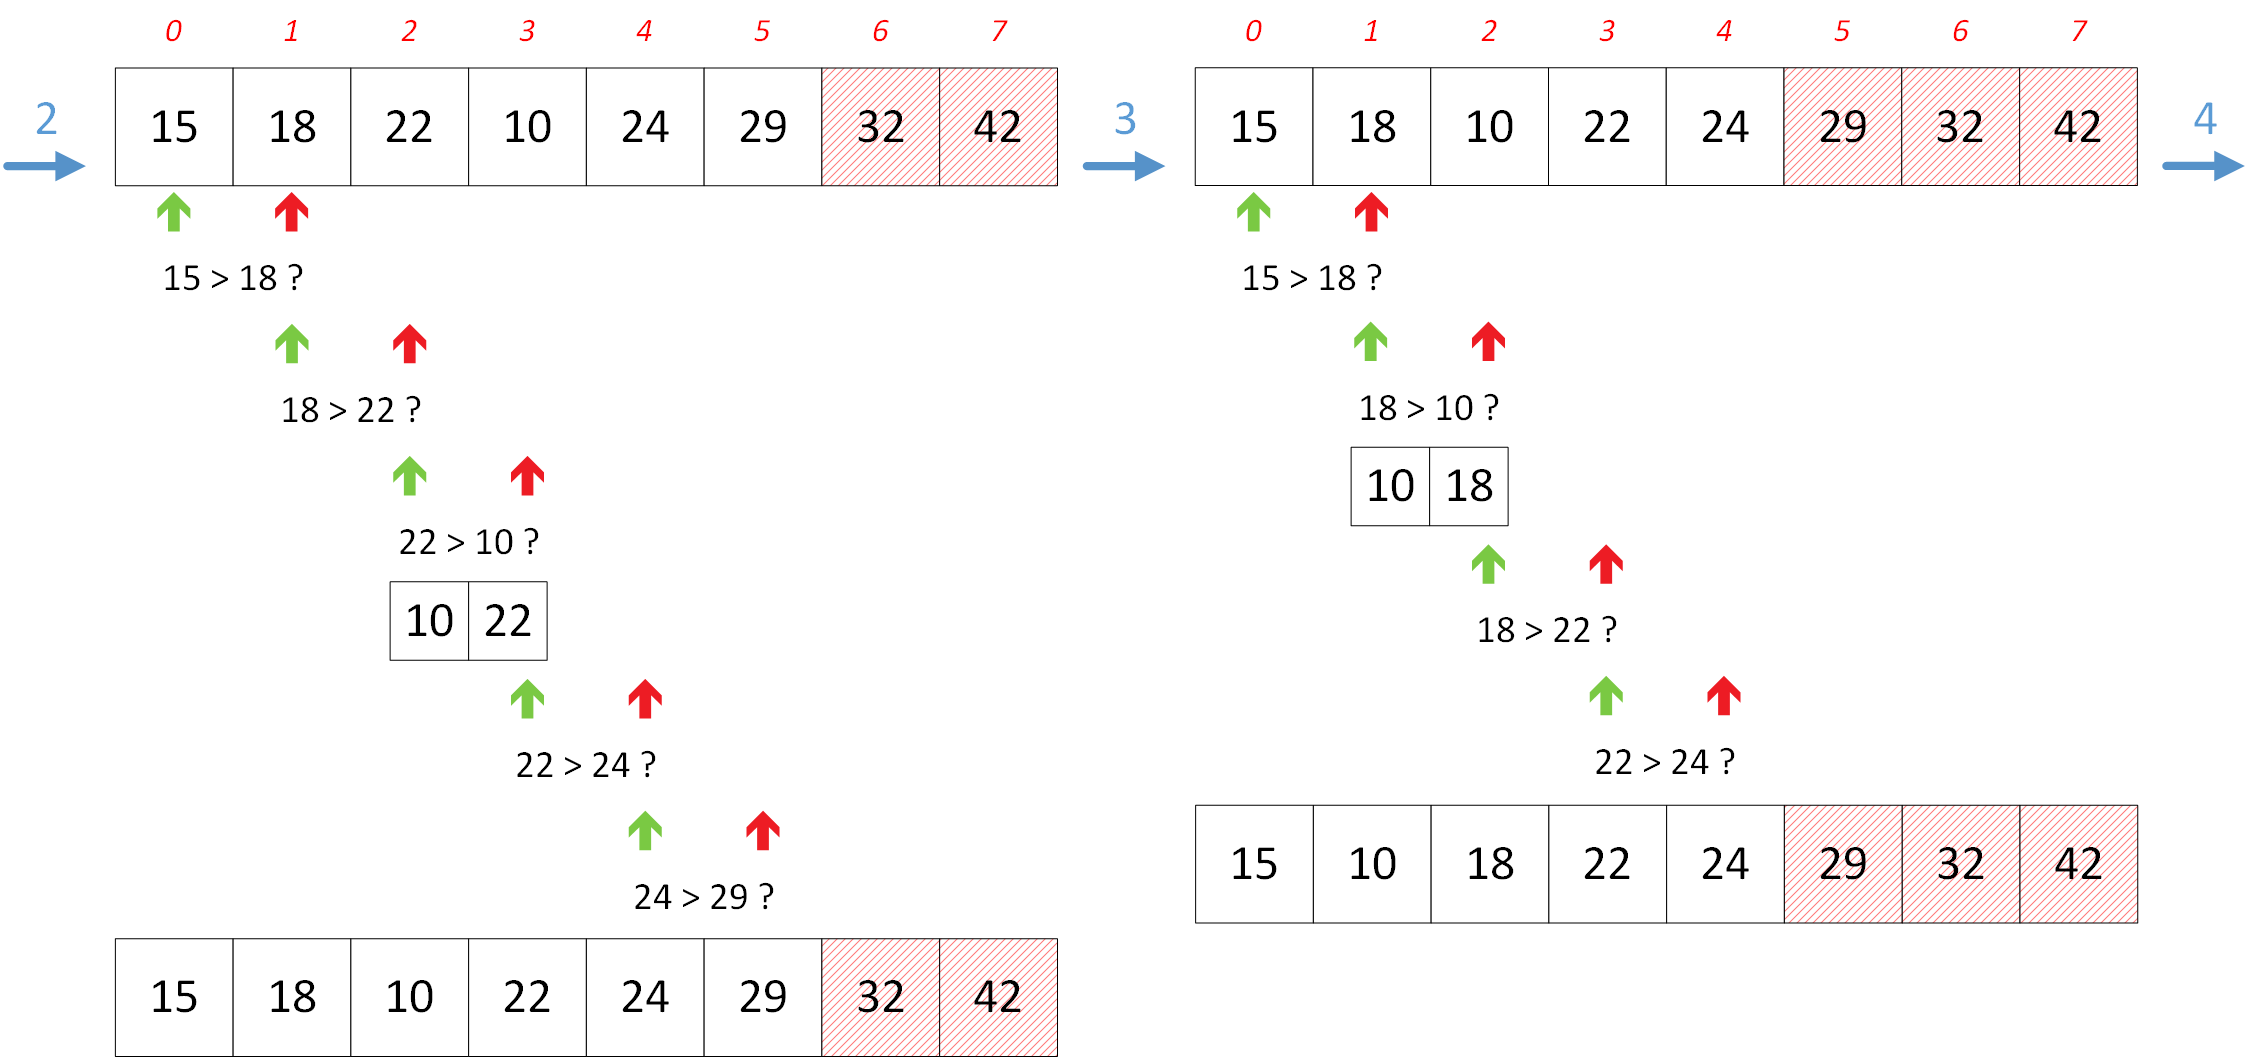
\includegraphics[width=1.2\textwidth]{img/tris/2_per_pages/BubbleSort_part2.png}
}
%\caption{Bubble Sort part 1}
%\label{figure:1-S3-DesignScience-ThreeLoops}
\end{figure}
%\end{figure*} % Figure flottante
% To use it : fig~\ref{label}

\vfillFirst

\par\rule{\textwidth}{0.5pt} 

\medskip

%\begin{figure*} % Figure flottante
\begin{figure}[ht!]
\centering
\centerline{
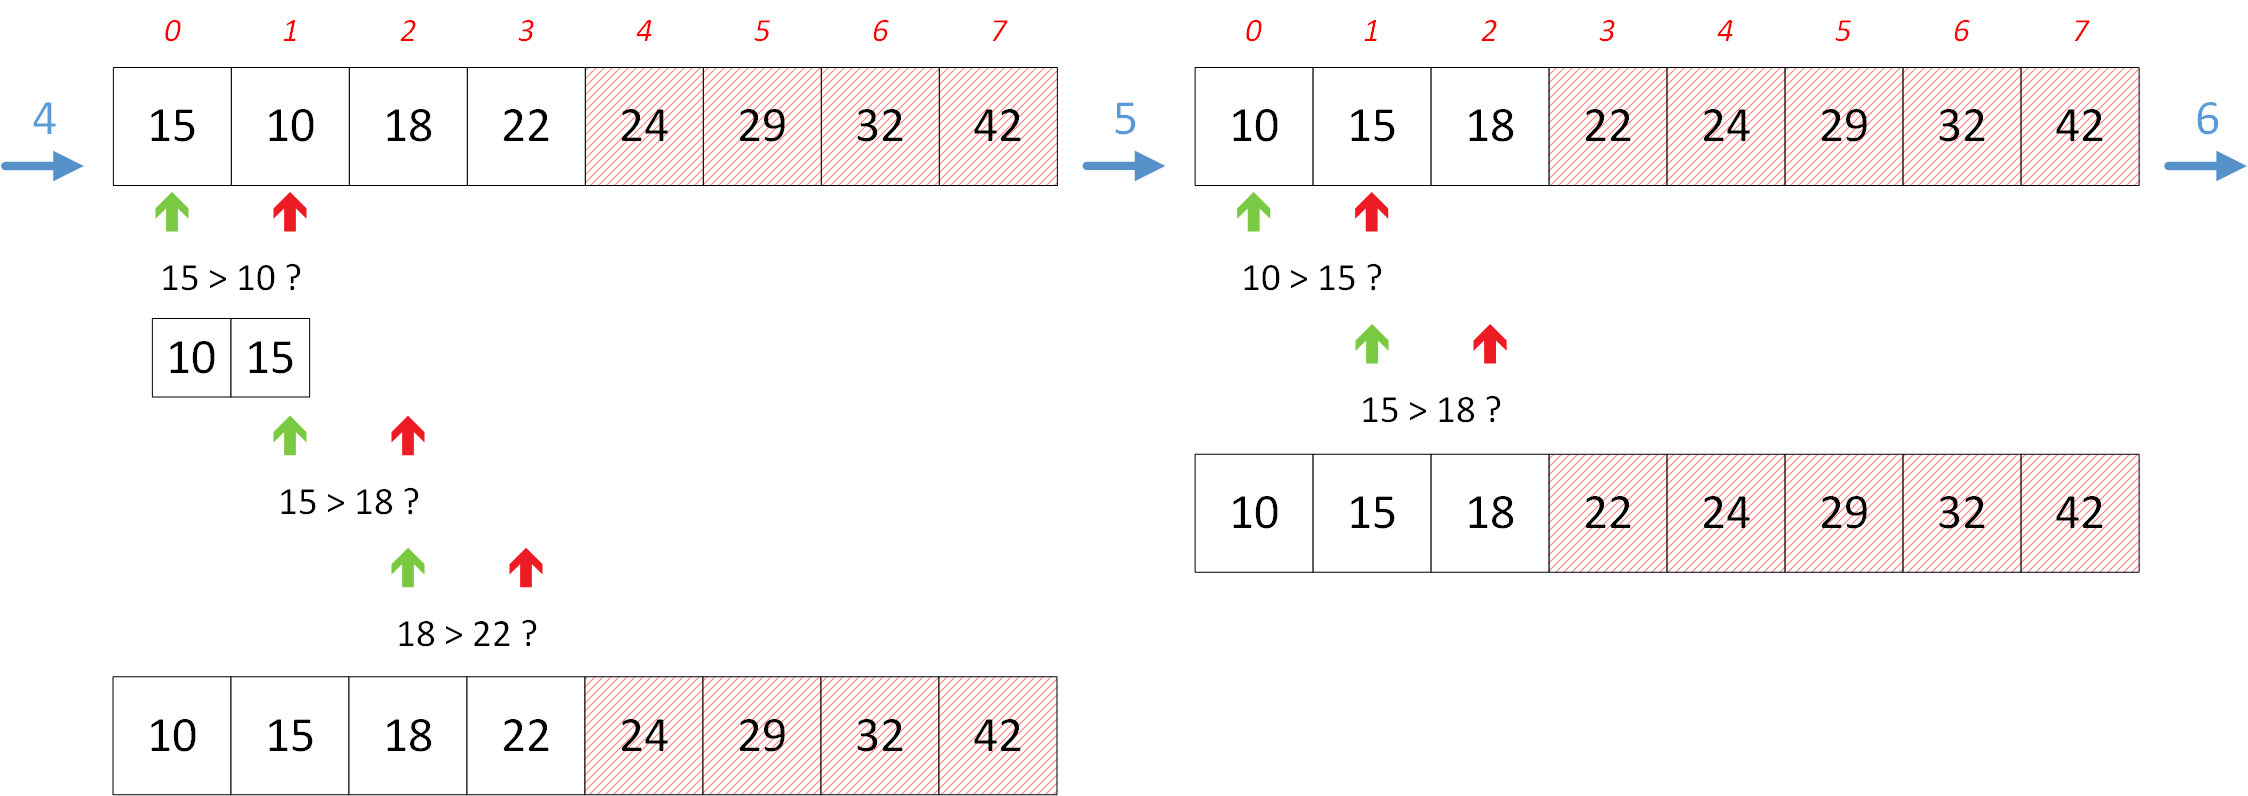
\includegraphics[width=1.2\textwidth]{img/tris/2_per_pages/BubbleSort_part3.png}
}
%\caption{Bubble Sort part 1}
%\label{figure:1-S3-DesignScience-ThreeLoops}
\end{figure}
%\end{figure*} % Figure flottante
% To use it : fig~\ref{label}

\medskip

\par\rule{\textwidth}{0.5pt} 

\vfillLast

%\begin{figure*} % Figure flottante
\begin{figure}[ht!]
\centering
\centerline{
%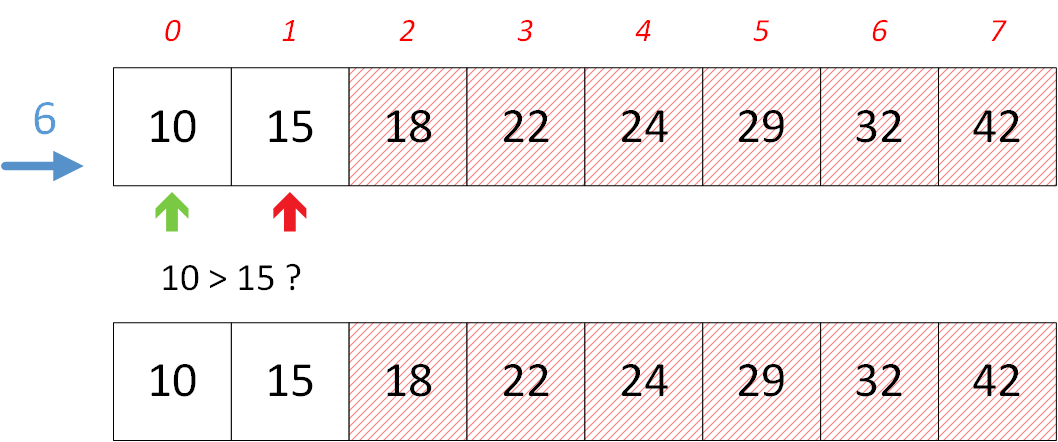
\includegraphics[scale=0.48]{img/tris/2_per_pages/BubbleSort_part4.png}
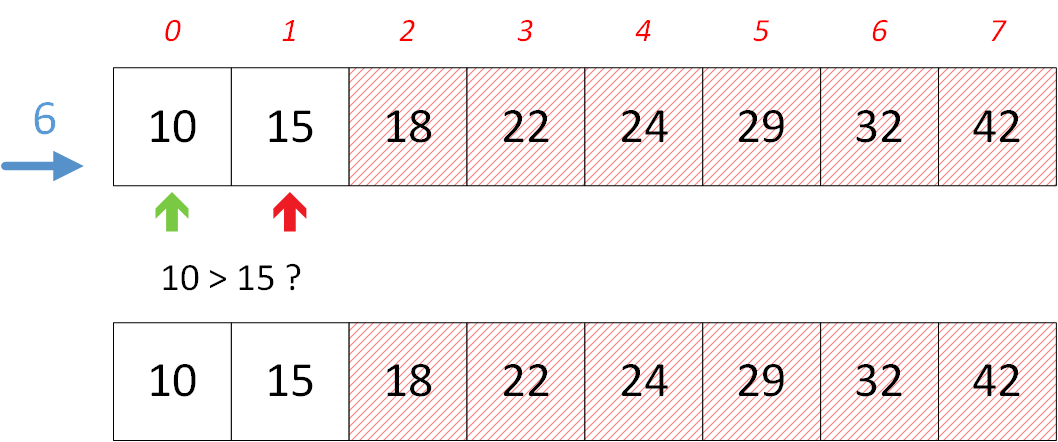
\includegraphics[width=0.6\textwidth]{img/tris/2_per_pages/BubbleSort_part4.png}
}
%\caption{Bubble Sort part 1}
%\label{figure:1-S3-DesignScience-ThreeLoops}
\end{figure}
%\end{figure*} % Figure flottante
% To use it : fig~\ref{label}


\bigskip

%\vfillFirst

\clearpage

Voici un exemple d'implémentation pour le tri à bulles :

\bigskip

\begin{table}[ht!]
  \centering
% %*   *)
\begin{lstlisting}[style=algorithmique]
algorithme procedure BubbleSort
  parametres locaux
    entier[]  tab
    entier    len
  variables
    entier    i, j
debut
pour i = (len - 1) %*\textbf{jusqu'a}*) 1 faire
  pour j = 0 %*\textbf{jusqu'a}*) (i - 1) faire
    si (tab[j] > tab[j + 1]) alors
      swap(tab, len, j, j + 1)
    fin si
  fin pour
fin pour
fin algorithme procedure BubbleSort \end{lstlisting}
%  \caption{Bla. }
%  \label{puissance}
\end{table}


Dans cette version du Bubble Sort, on va chercher à pousser les plus gros éléments à la fin à chaque fois en faisant avancer chaque élément plus grand vers la droite.
Une fois que le plus grand élément a été trouvé, il est naturellement poussé vers la droite.
Une fois que ce plus grand élément est poussé à la fin du tableau, plus aucun élément ne sera plus grand, donc inutile de les comparer avec.
Ainsi, la dernière case la plus à droite devient immuable.

\medskip

La première boucle avec \textbf{i} permet de déterminer quelle colonne va servir de fin pour les balayages successifs, et à chaque itération, on n'ira pas plus loin.
La boucle utilisant \textbf{j} permet d'effectuer les balayages successifs et d'échanger la position entre un élément courant et son suivant s'il est plus petit.
Ainsi, en tombant sur le plus grand élément, on va le déplacer progressivement jusqu'à la fin du tableau.
On recommence avec les éléments restants, donc avec le deuxième plus grand, et ainsi de suite.

%\bigskip
%\clearpage
\vfillFirst
\vfillLast

%%%%%%%%%%%%%%%%%%%%%%%%%%%%%%%%%%%

\section{Tri par Sélection}

\medskip

Le tri par sélection est le tri le plus évident humainement parlant : il suffit de chercher à chaque tour le plus grand élément restant, pour le placer en fin de tableau.

\medskip

On cherche donc la valeur la plus grande en parcourant toutes les cases, puis, on échange la place de cet élément avec le tout dernier du tableau (pour le mettre à sa place définitive).
Et on recommence ce traitement (sans lire la dernière case à chaque fois) jusqu'à avoir ordonné tous les éléments.

\medskip

\begin{itemize}
\item Complexité moyenne : $ T(n) = O(n^{2}) $
\item Complexité pire cas : $ T(n) = O(n^{2}) $
\item Complexité meilleur cas : $ T(n) = O(n^{2}) $
\item Tri en place
\item Tri instable
\end{itemize}


%\medskip
\clearpage


\vfillFirst

%\begin{figure*} % Figure flottante
\begin{figure}[ht!]
\centering
\centerline{
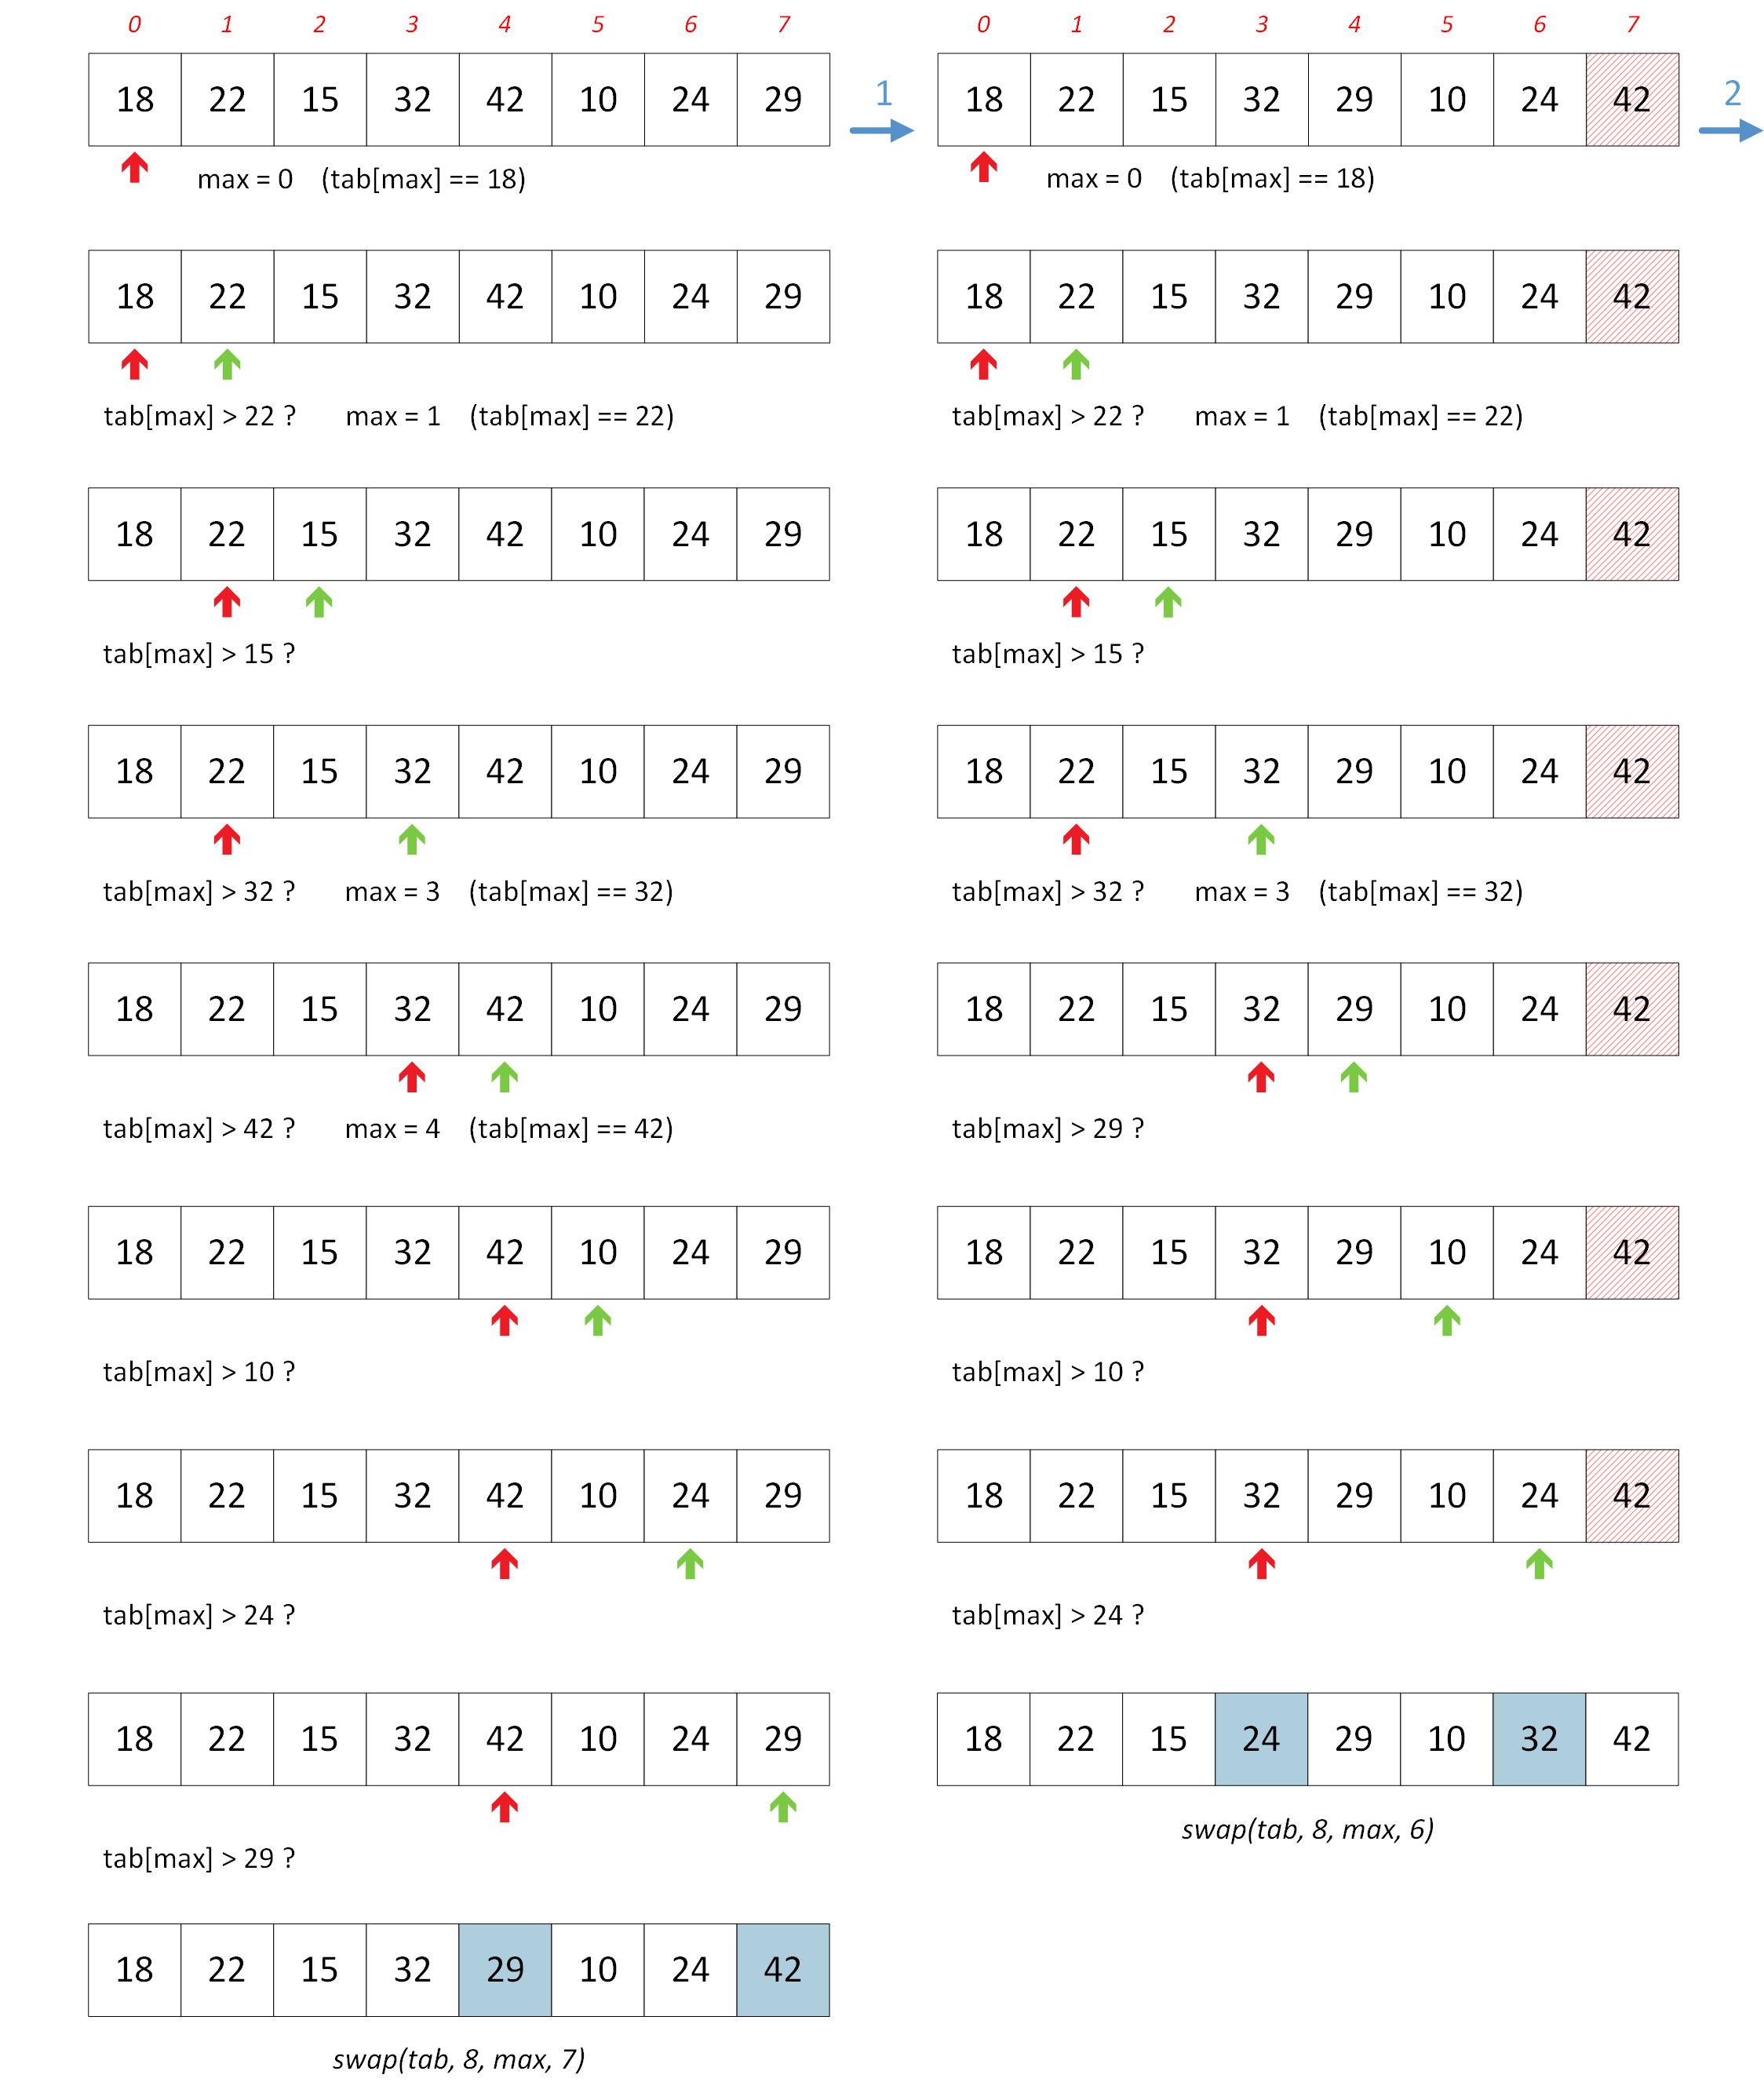
\includegraphics[width=1.2\textwidth]{img/tris/2_per_pages/SelectionSort_part1.png}
}
%\caption{Bubble Sort part 1}
%\label{figure:1-S3-DesignScience-ThreeLoops}
\end{figure}
%\end{figure*} % Figure flottante
% To use it : fig~\ref{label}

\vfill

%\vfillLast

\clearpage

\vfillFirst

%\begin{figure*} % Figure flottante
\begin{figure}[ht!]
\centering
\centerline{
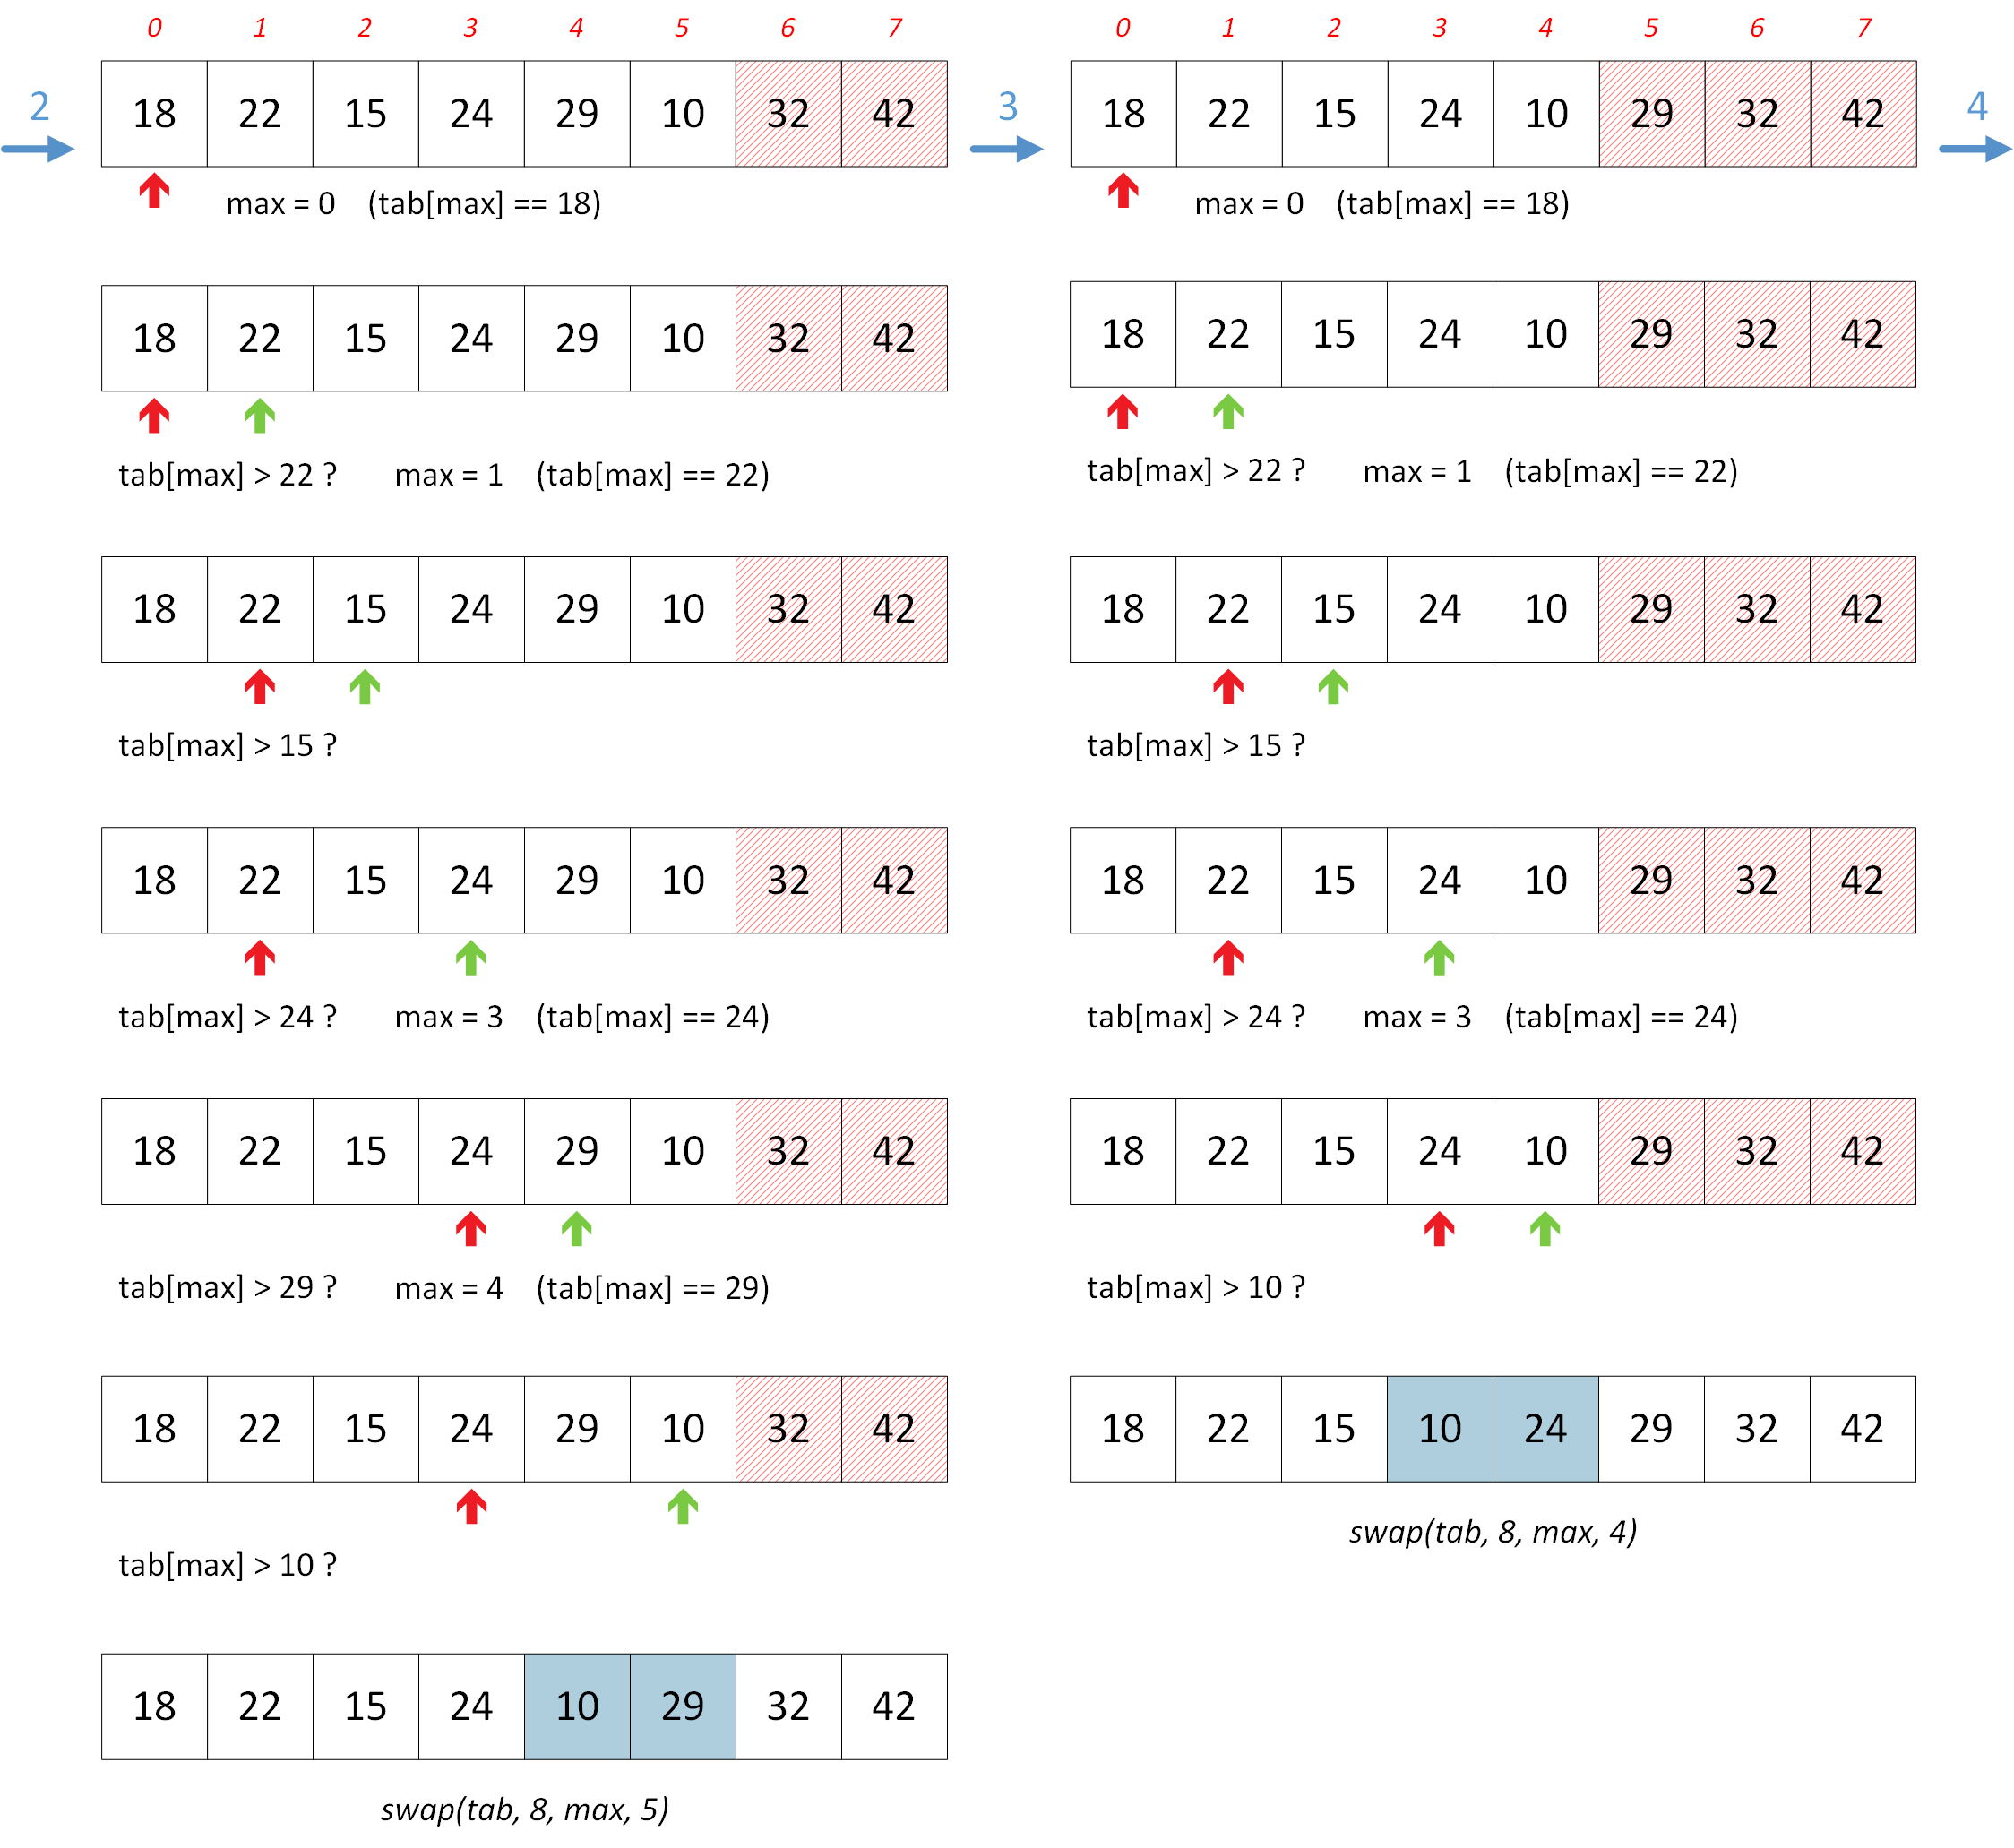
\includegraphics[width=1.2\textwidth]{img/tris/2_per_pages/SelectionSort_part2.png}
}
%\caption{Bubble Sort part 1}
%\label{figure:1-S3-DesignScience-ThreeLoops}
\end{figure}
%\end{figure*} % Figure flottante
% To use it : fig~\ref{label}

\vfillLast

\clearpage

%\begin{figure*} % Figure flottante
\begin{figure}[ht!]
\centering
\centerline{
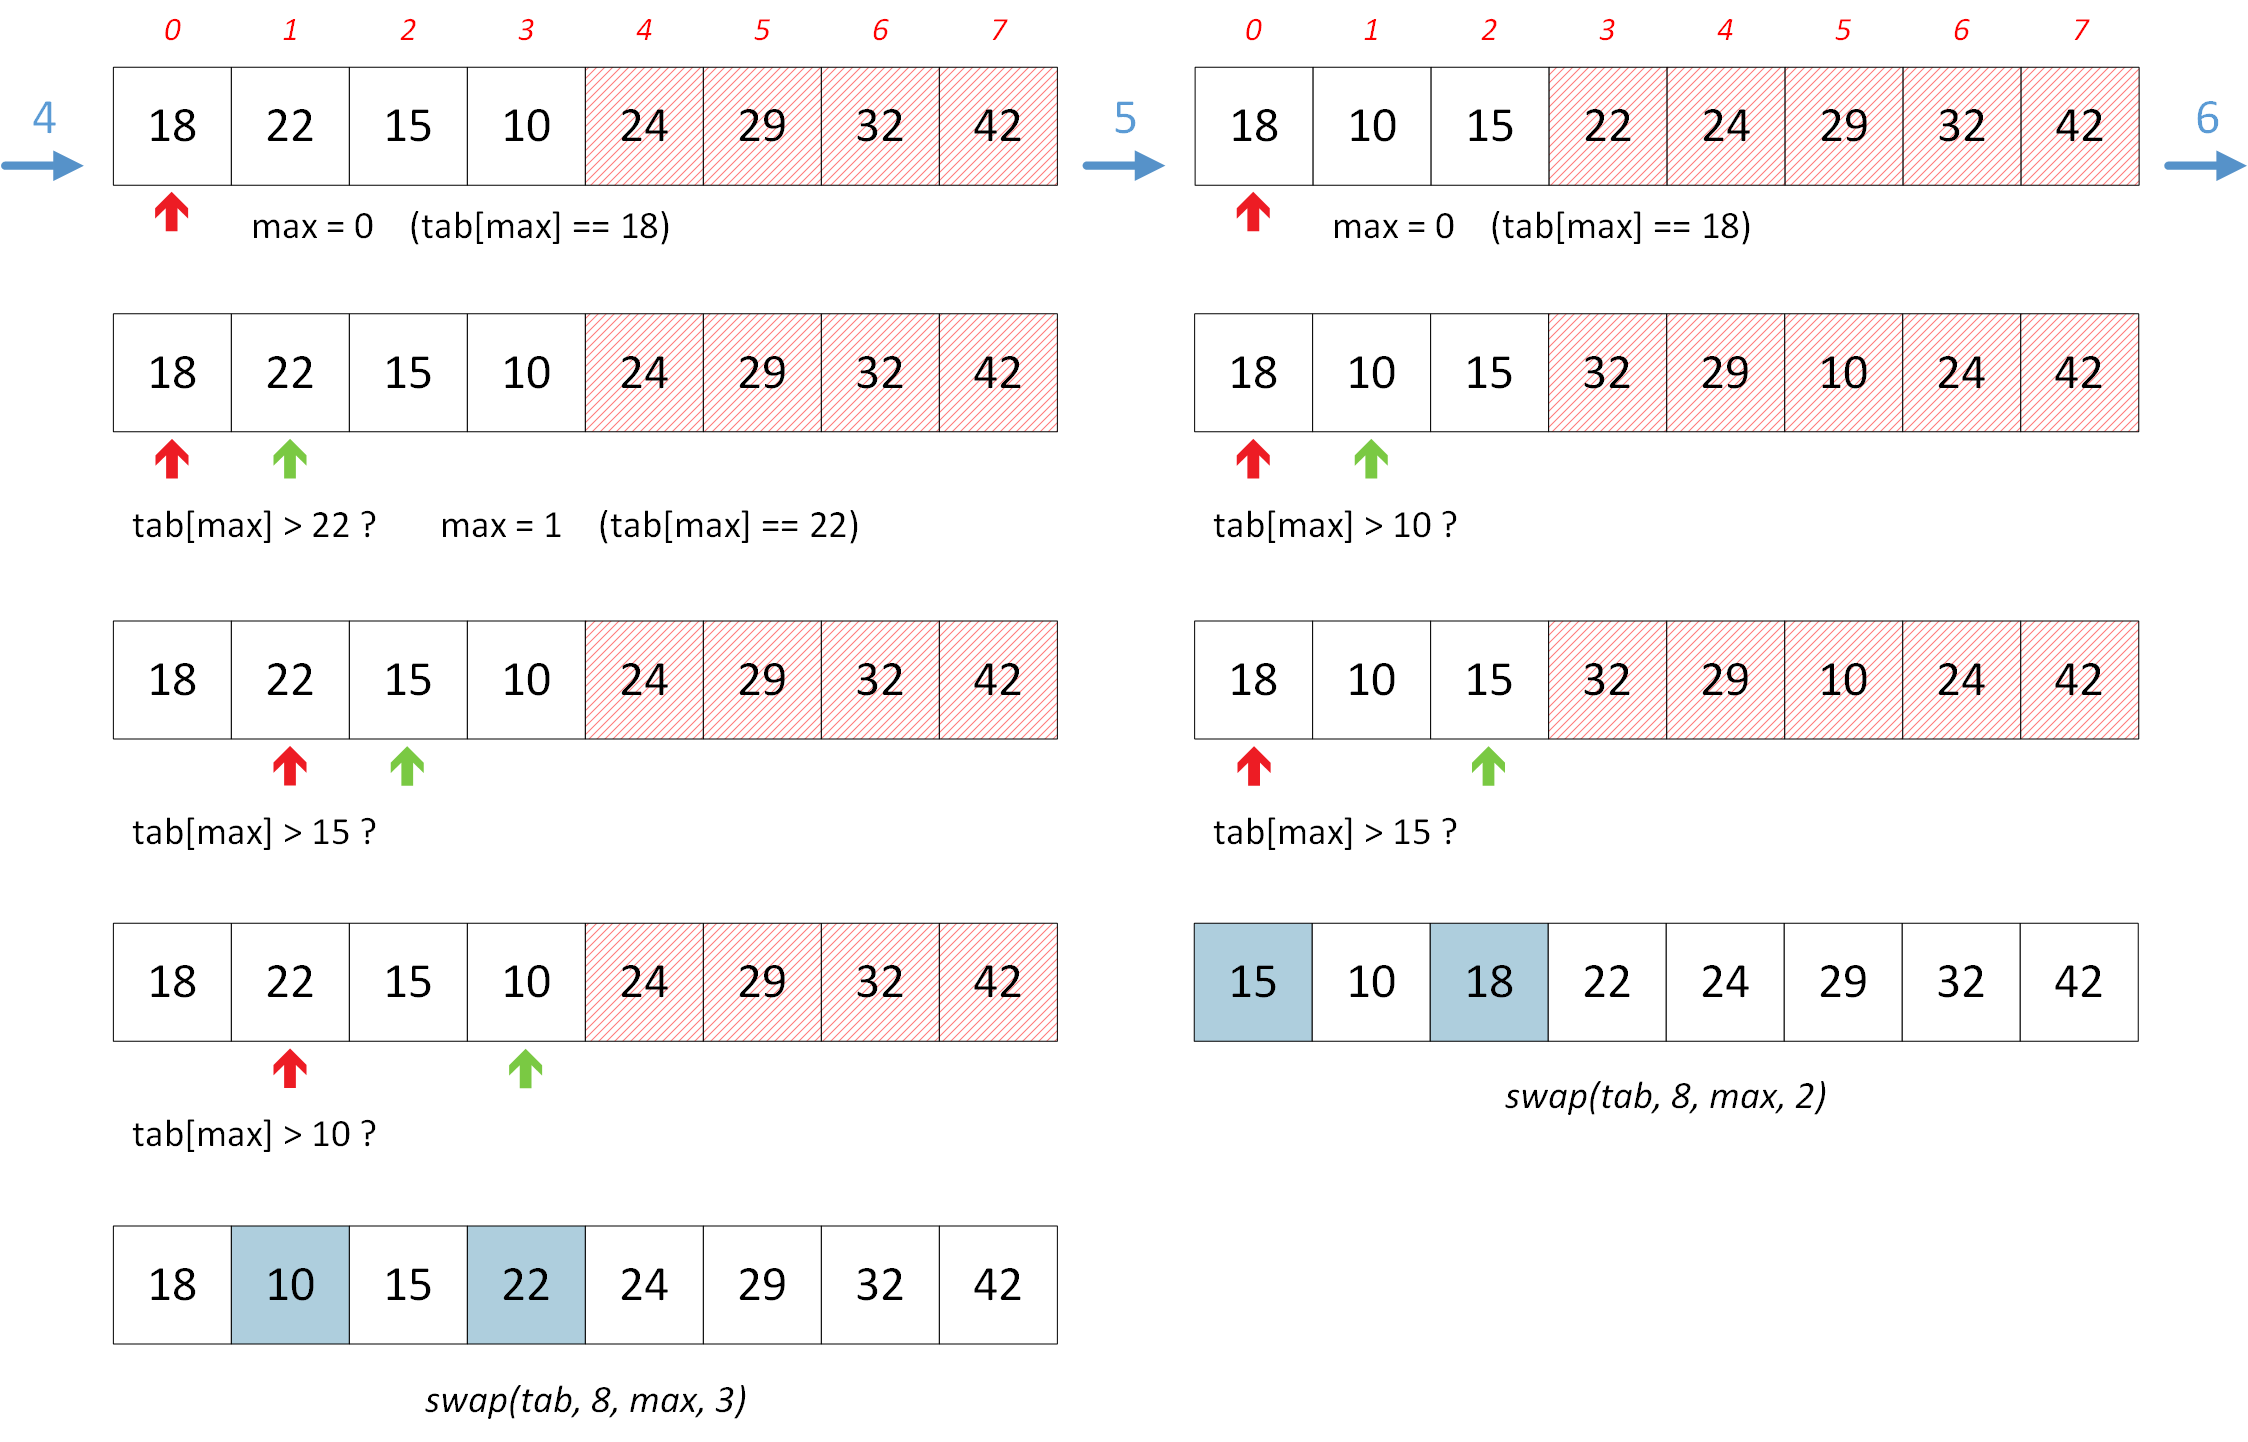
\includegraphics[width=1.2\textwidth]{img/tris/2_per_pages/SelectionSort_part3.png}
}
%\caption{Bubble Sort part 1}
%\label{figure:1-S3-DesignScience-ThreeLoops}
\end{figure}
%\end{figure*} % Figure flottante
% To use it : fig~\ref{label}

\vfillFirst

\par\rule{\textwidth}{0.5pt} 

\vfillLast

%\begin{figure*} % Figure flottante
\begin{figure}[ht!]
\centering
\centerline{
%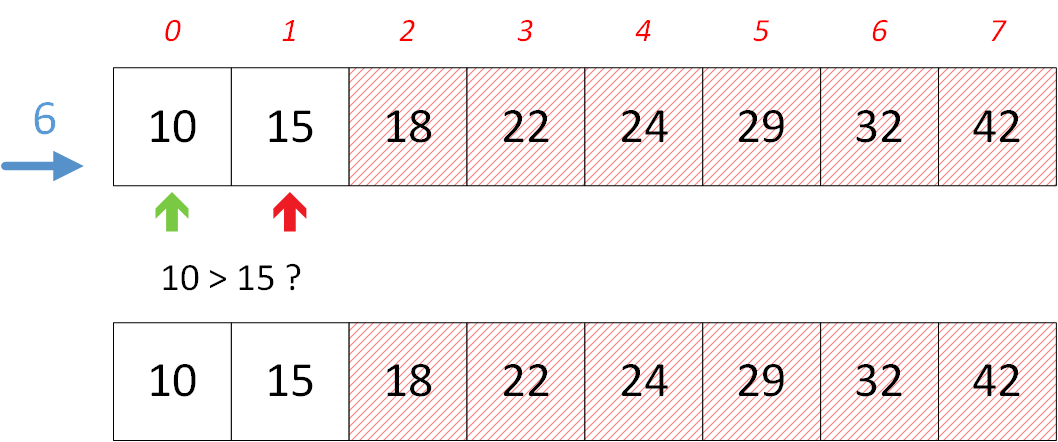
\includegraphics[scale=0.48]{img/tris/2_per_pages/BubbleSort_part4.png}
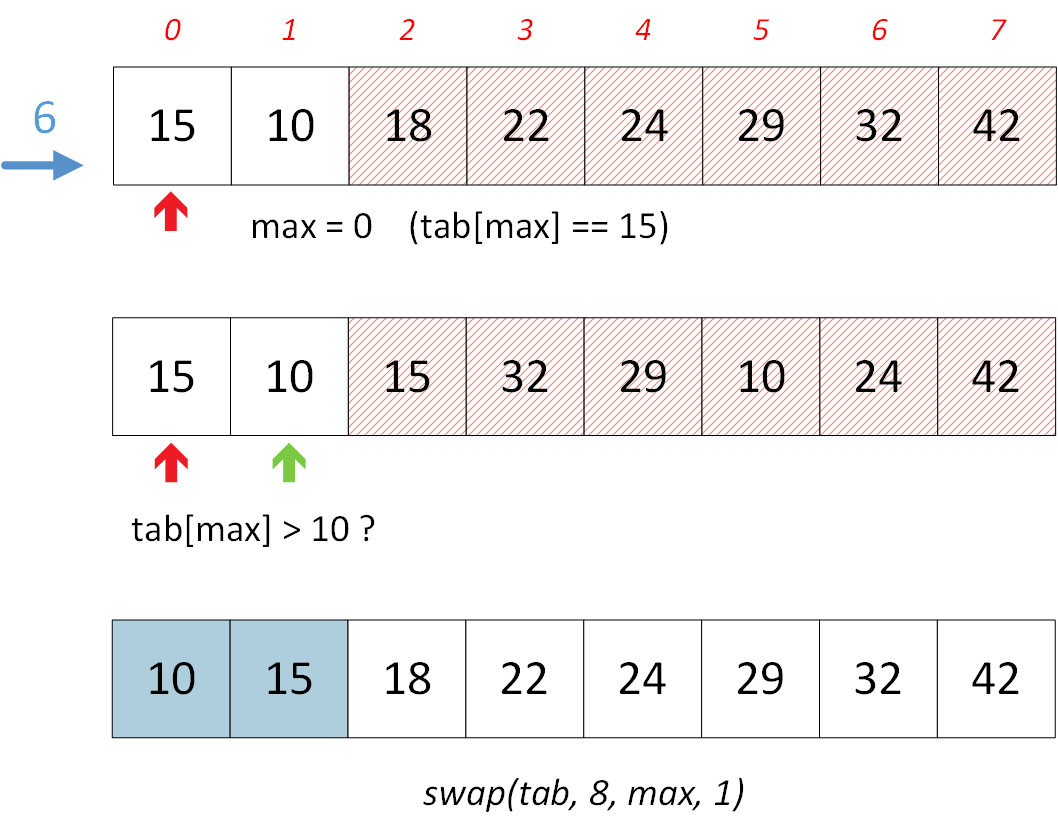
\includegraphics[width=0.6\textwidth]{img/tris/2_per_pages/SelectionSort_part4.png}
}
%\caption{Bubble Sort part 1}
%\label{figure:1-S3-DesignScience-ThreeLoops}
\end{figure}
%\end{figure*} % Figure flottante
% To use it : fig~\ref{label}


%\bigskip
\clearpage

Voici un exemple d'implémentation pour le tri par sélection :

\bigskip

\begin{table}[ht!]
  \centering
% %*   *)
\begin{lstlisting}[style=algorithmique]
algorithme procedure SelectionSort
  parametres locaux
    entier[]  tab
    entier    len
  variables
    entier    max_range, max
debut
pour max_range = (len - 1) %*\textbf{jusqu'a}*) 2 faire
  max = 0
  pour i = 1 %*\textbf{jusqu'a}*) (max_range) faire
    si (tab[i] > tab[max]) alors
      max = i
    fin si
  fin pour
  swap(tab, len, max, max_range)
fin pour
fin algorithme procedure SelectionSort \end{lstlisting}
%  \caption{Bla. }
%  \label{puissance}
\end{table}

Il s'agit du cas général permettant de parcourir le tableau plusieurs fois.
\`A chaque parcours, on cherche la valeur la plus grande, et on la place à la fin.
\'Etant donné que le plus grand élément est placé en fin, on va réduire le parcours d'un élément à chaque fois.
Ainsi, le premier parcours fera la longueur du tableau, le dernier parcours ne fera que comparer les 2 premiers éléments pour placer correctement les deux plus petits éléments du tableau.

\medskip

Cet algorithme a l'inconvénient de nécessiter au moins 3 éléments dans le tableau pour fonctionner correctement.
Ainsi, on peut soit faire une fonction chapeau testant les cas où la longueur est inférieure à 3, soit ajouter un pré-traitement dans la fonction.

\bigskip

\begin{table}[ht!]
  \centering
% %*   *)
\begin{lstlisting}[style=algorithmique]
algorithme procedure PreProcessingSelectionSort
  parametres locaux
    entier[]  tab
    entier    len
debut
si (len >= 2) alors
  si (len == 2) alors
    si (tab[0] > tab[1]) alors
      swap(tab, len, 0, 1)
    fin si
  sinon
    SelectionSort(tab, len)
  fin si
fin si
fin algorithme procedure PreProcessingSelectionSort \end{lstlisting}
%  \caption{Bla. }
%  \label{puissance}
\end{table}


\clearpage
%\bigskip

%%%%%%%%%%%%%%%%%%%%%%%%%%%%%%%%%%%

\section{Tri par Insertion}

\medskip

Le tri par insertion considère que le tableau donné en paramètre n'est pas trié, et seuls les éléments qu'il a manipulé successivement le sont.
Ainsi, chaque élément du tableau est comparé à tous ceux déjà triés, et on le place là où il devrait être.

\medskip

Pour le premier élément, celui-ci est considéré comme déjà trié, on peut donc passer au deuxième.
Le deuxième est comparé avec l'unique élément déjà trié : on échange leurs deux places si nécessaire.
Le troisième élément est comparé au plus grand des deux éléments triés, s'il est plus grand ou égal, il reste à sa place, sinon on le décale vers la gauche d'un cran, et on le compare à l'élément suivant (et ainsi de suite pour trouver sa place finale).

\medskip

Chaque élément du tableau est donc \textit{inséré} à sa place parmi les éléments considérés comme triés.

\medskip

\begin{itemize}
\item Complexité moyenne : $ T(n) = O(n^{2}) $
\item Complexité pire cas : $ T(n) = O(n^{2}) $
\item Complexité meilleur cas : $ T(n) = O(n) $
\item Tri en place
\item Tri stable
\end{itemize}


%\medskip

\vfillFirst
\vfillLast


%\begin{figure*} % Figure flottante
\begin{figure}[ht!]
\centering
\centerline{
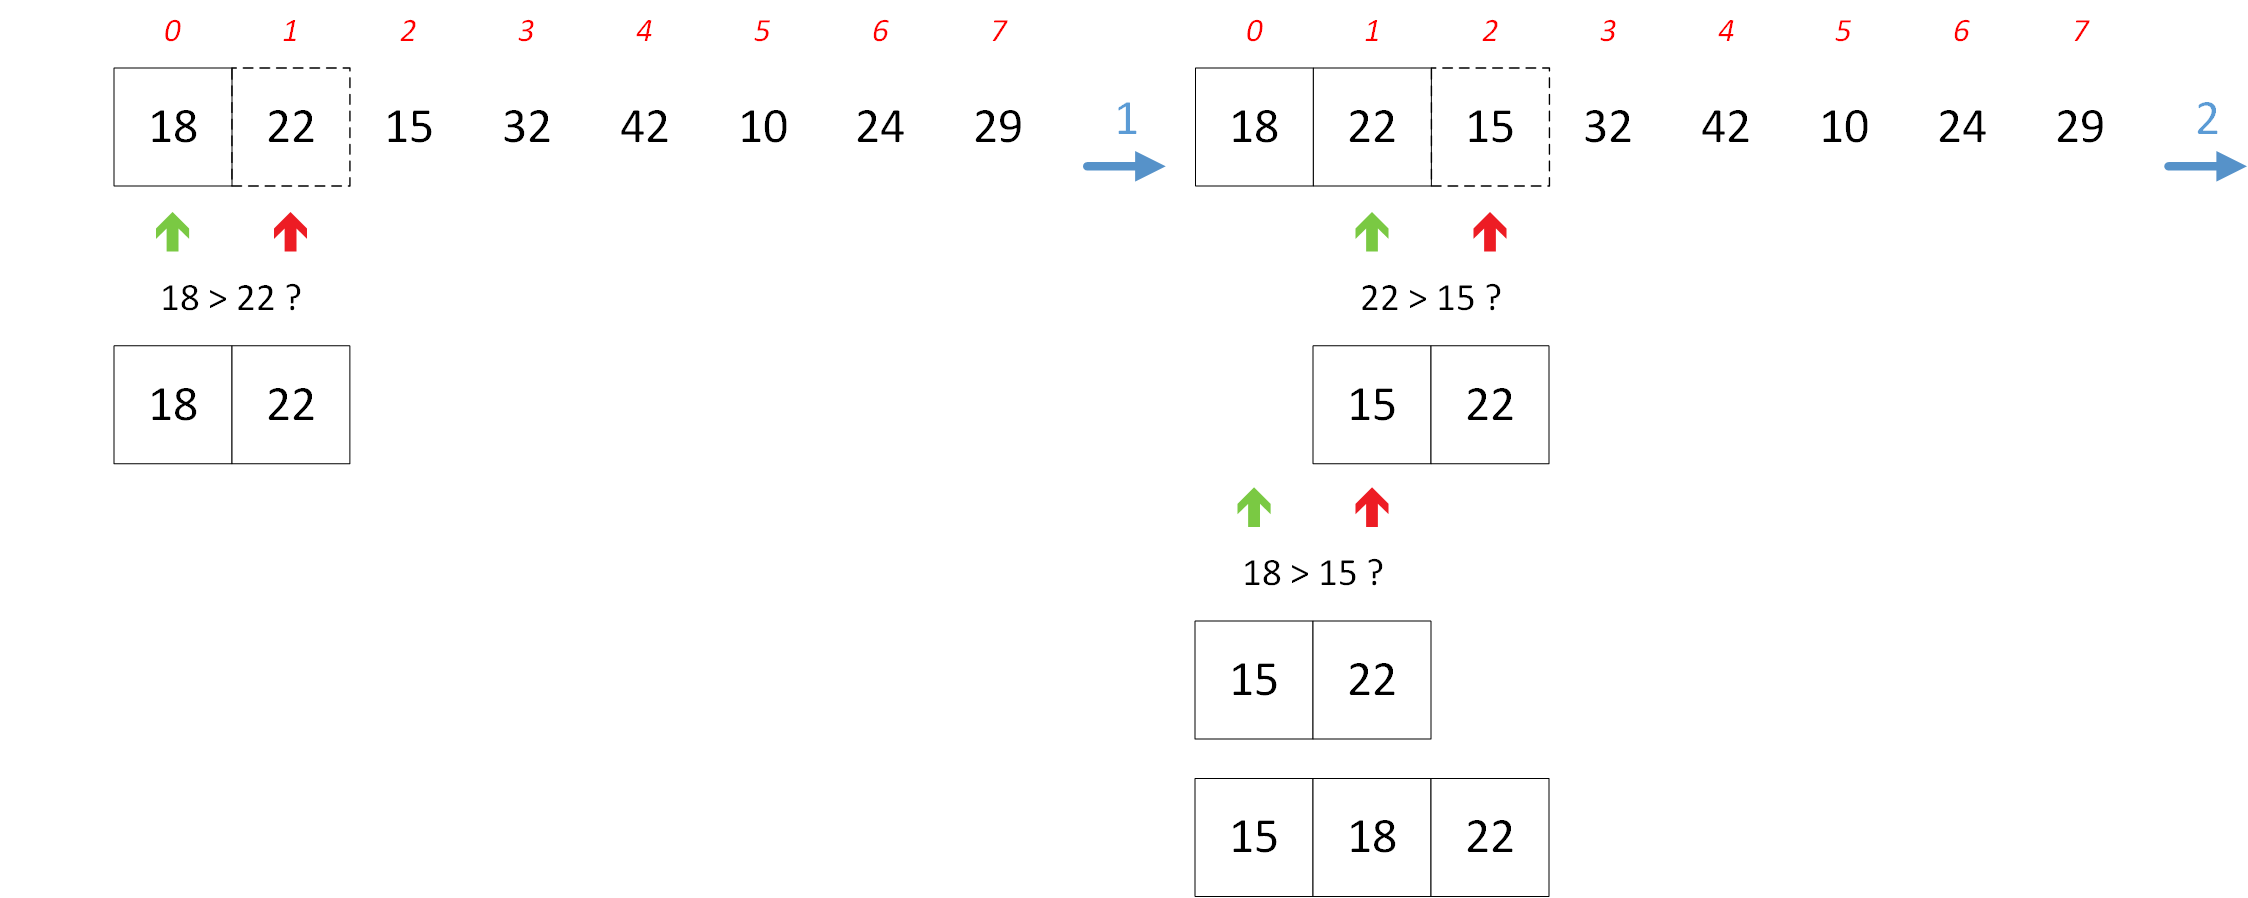
\includegraphics[width=1.2\textwidth]{img/tris/2_per_pages/InsertionSort_part1.png}
}
%\caption{Bubble Sort part 1}
%\label{figure:1-S3-DesignScience-ThreeLoops}
\end{figure}
%\end{figure*} % Figure flottante
% To use it : fig~\ref{label}

\medskip

\par\rule{\textwidth}{0.5pt} 

\medskip

%\begin{figure*} % Figure flottante
\begin{figure}[ht!]
\centering
\centerline{
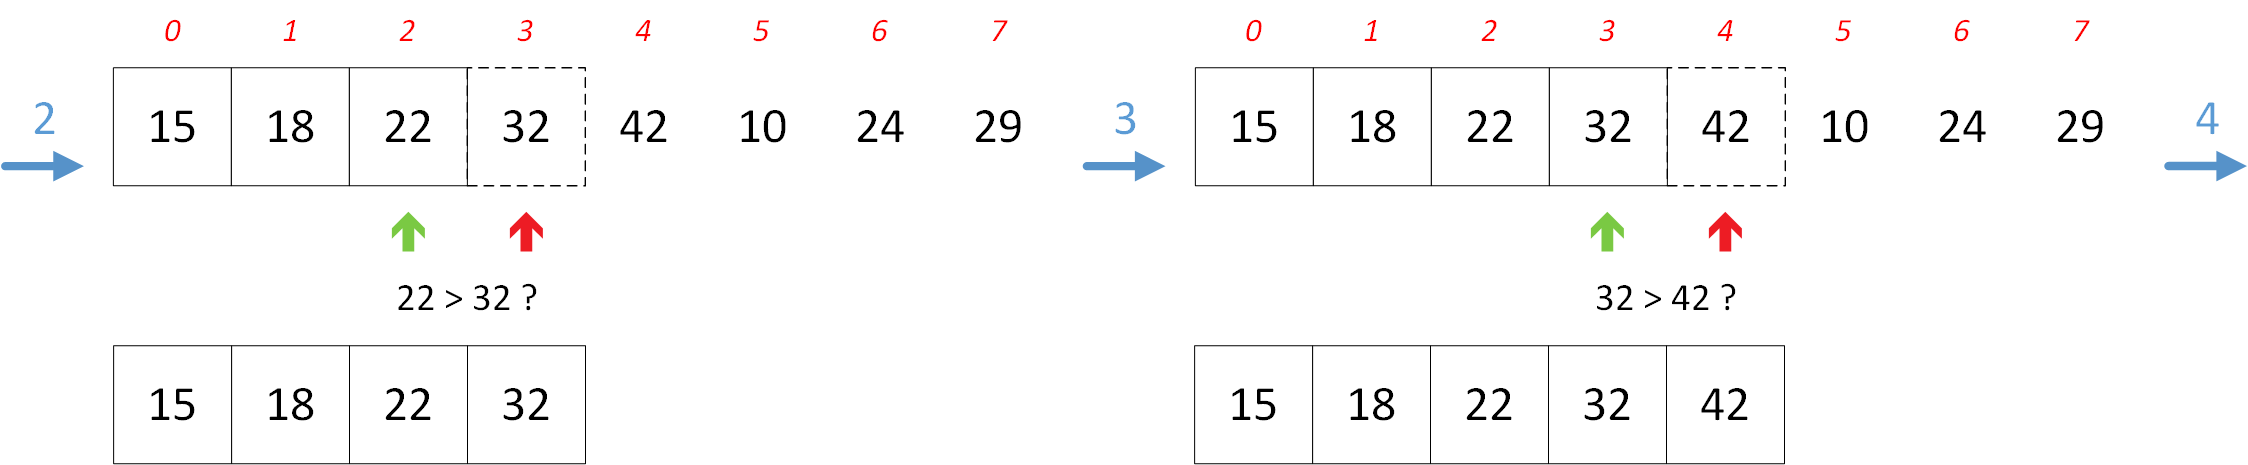
\includegraphics[width=1.2\textwidth]{img/tris/2_per_pages/InsertionSort_part2.png}
}
%\caption{Bubble Sort part 1}
%\label{figure:1-S3-DesignScience-ThreeLoops}
\end{figure}
%\end{figure*} % Figure flottante
% To use it : fig~\ref{label}

\clearpage

\vfillFirst

%\begin{figure*} % Figure flottante
\begin{figure}[ht!]
\centering
\centerline{
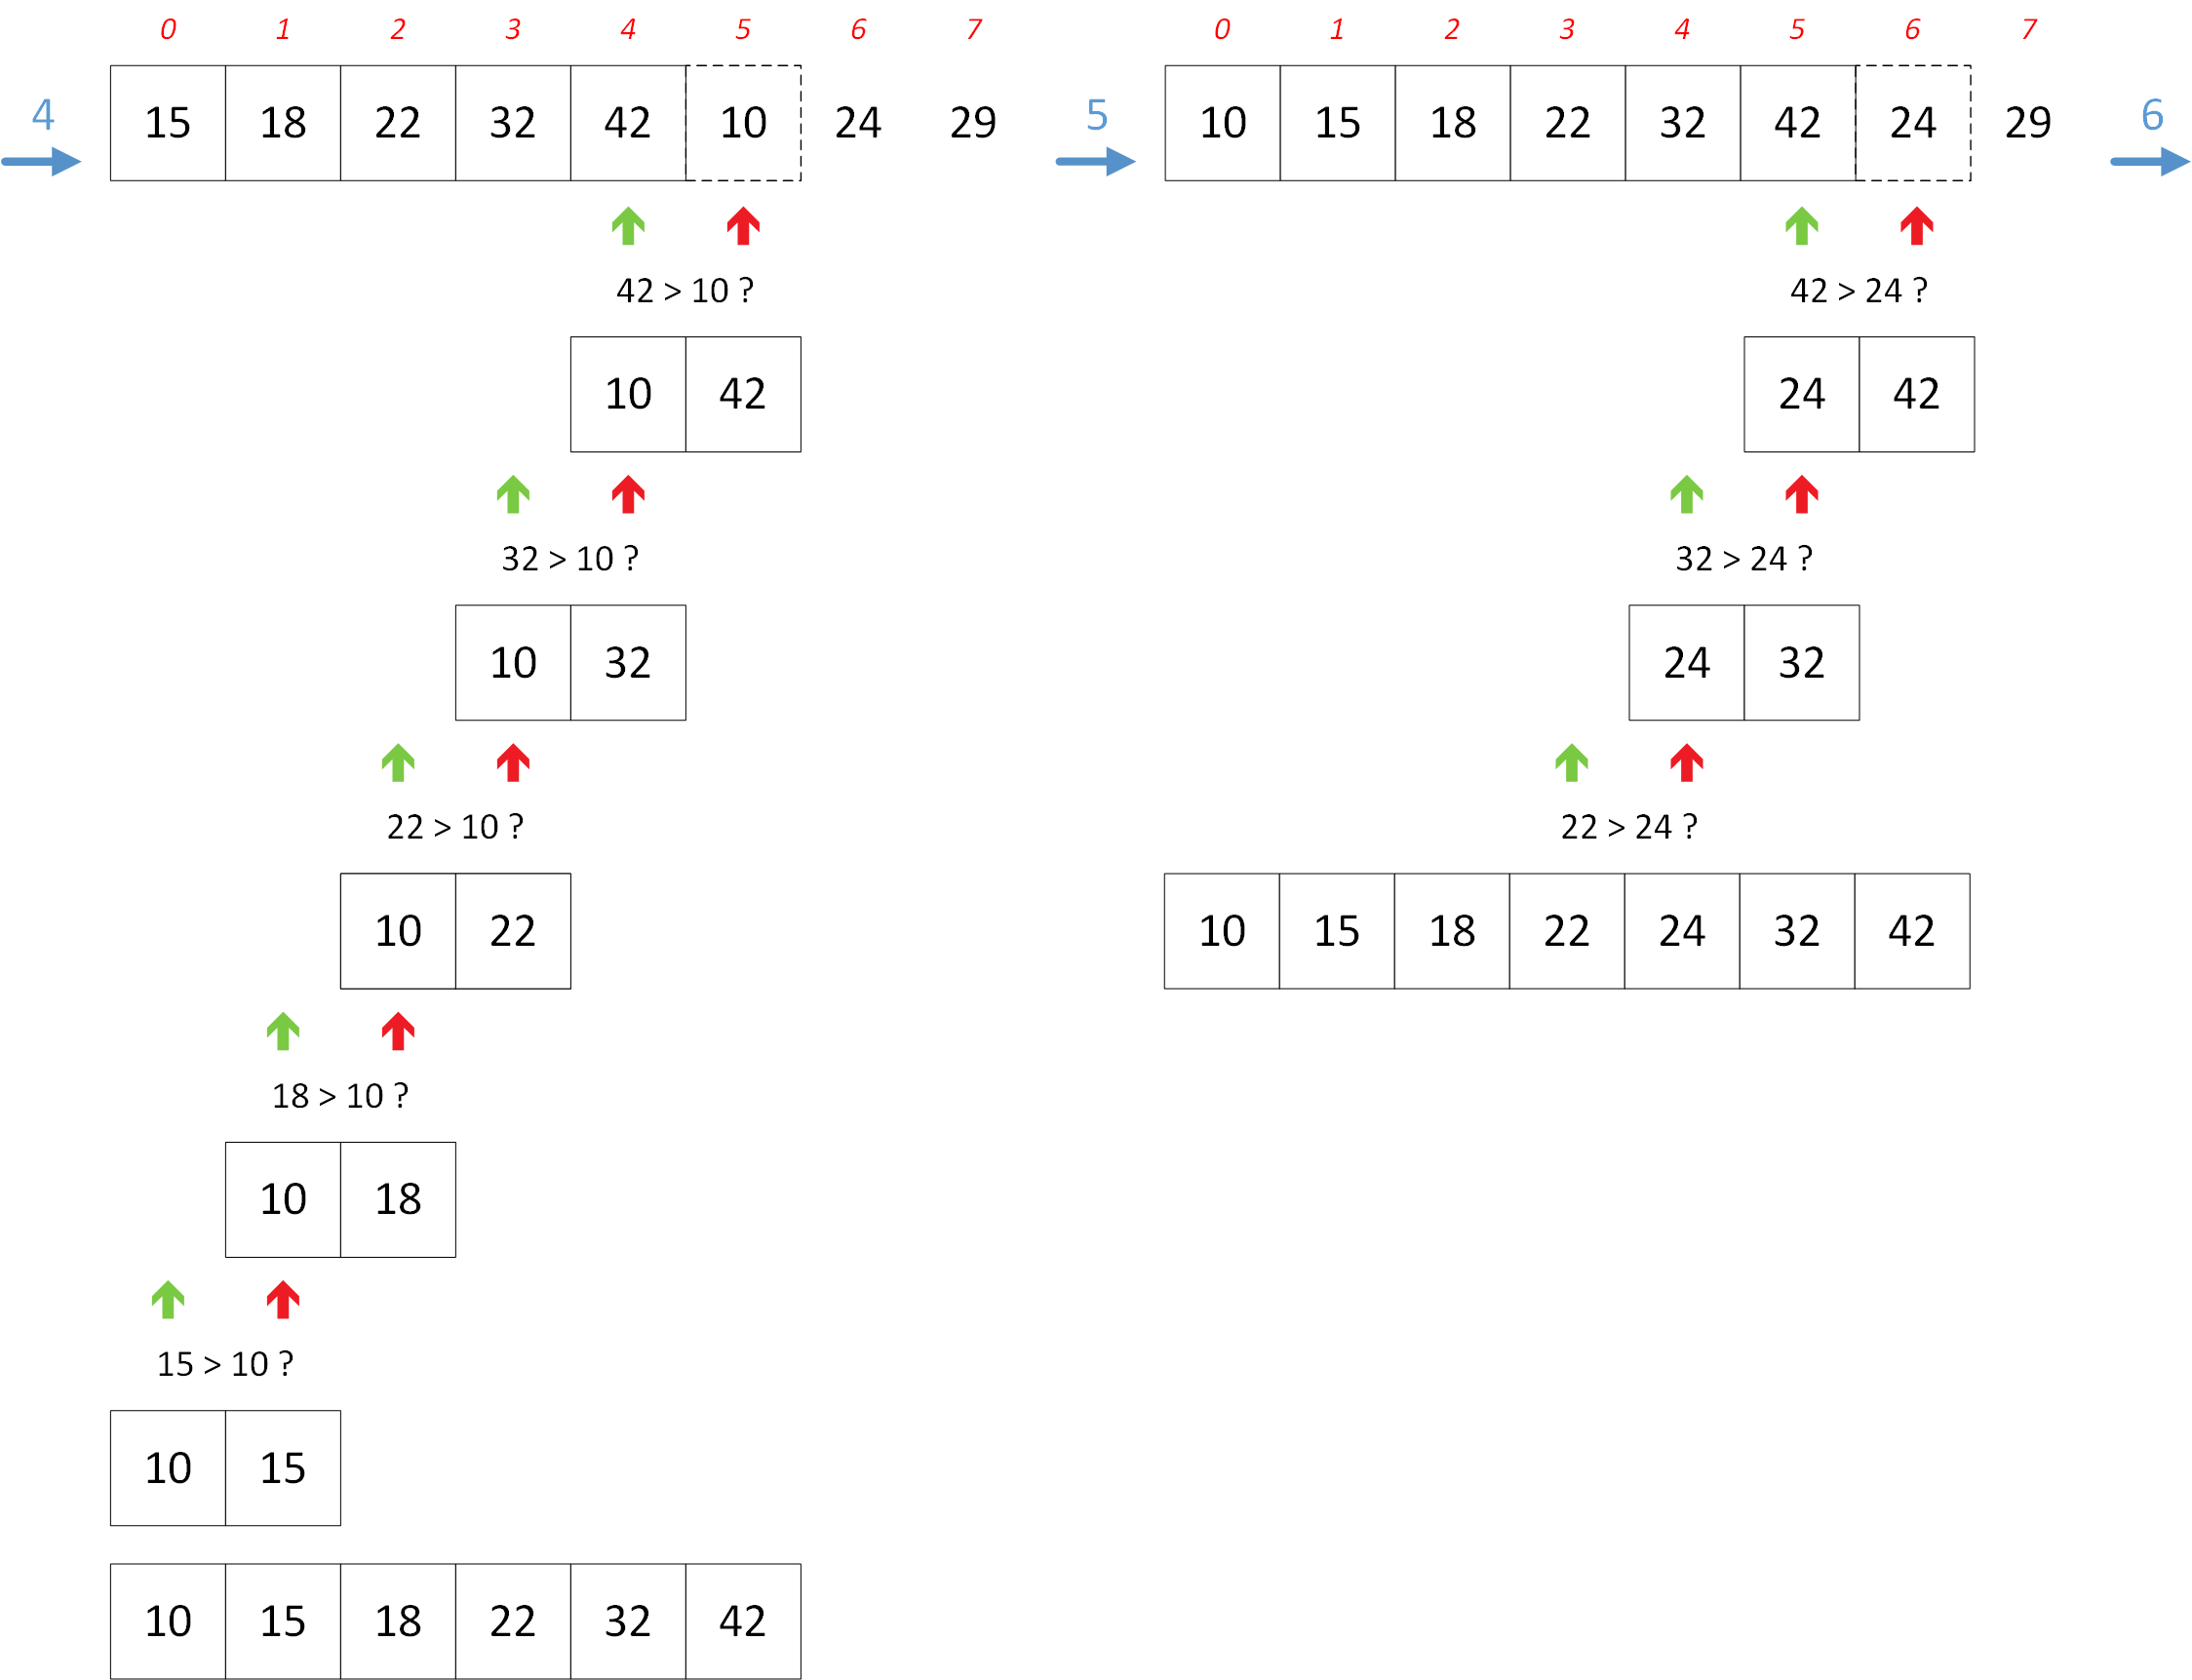
\includegraphics[width=1.2\textwidth]{img/tris/2_per_pages/InsertionSort_part3.png}
}
%\caption{Bubble Sort part 1}
%\label{figure:1-S3-DesignScience-ThreeLoops}
\end{figure}
%\end{figure*} % Figure flottante
% To use it : fig~\ref{label}

\vfillLast

\clearpage

%\begin{figure*} % Figure flottante
\begin{figure}[ht!]
\centering
\centerline{
%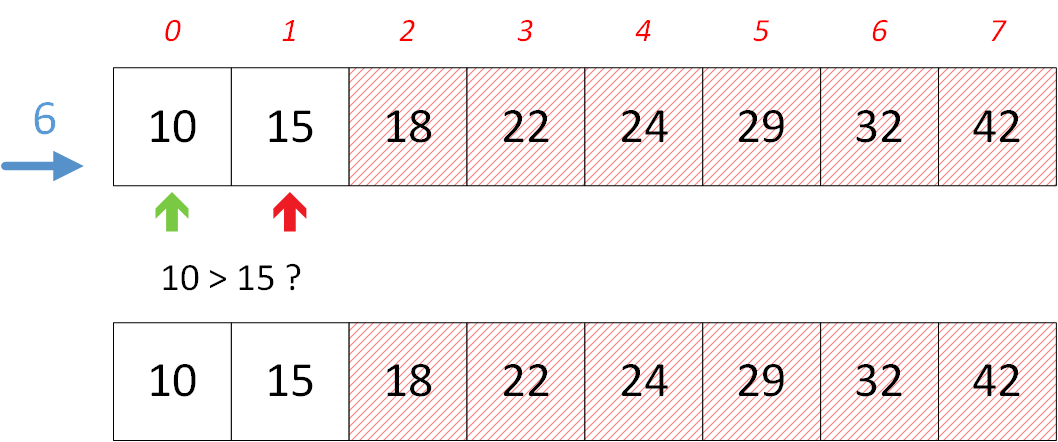
\includegraphics[scale=0.48]{img/tris/2_per_pages/BubbleSort_part4.png}
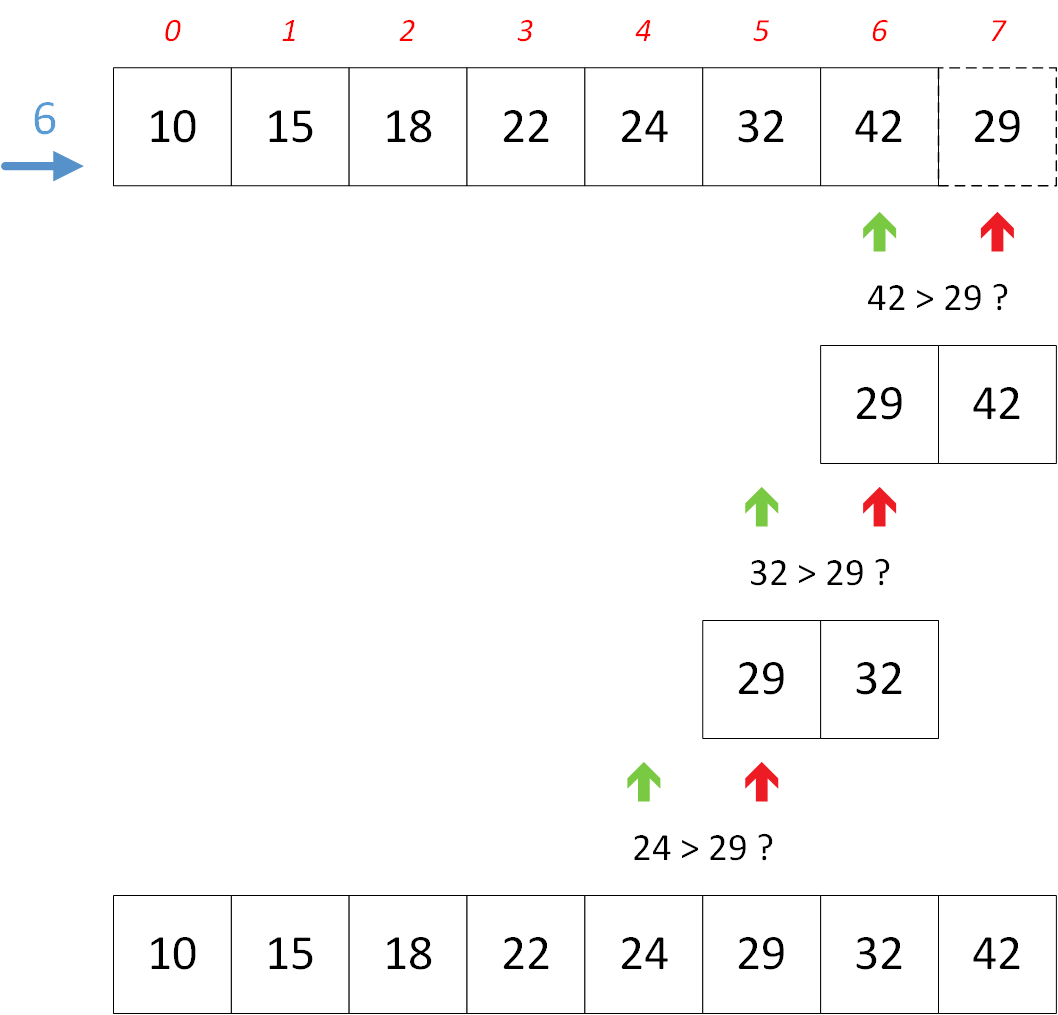
\includegraphics[width=0.6\textwidth]{img/tris/2_per_pages/InsertionSort_part4.png}
}
%\caption{Bubble Sort part 1}
%\label{figure:1-S3-DesignScience-ThreeLoops}
\end{figure}
%\end{figure*} % Figure flottante
% To use it : fig~\ref{label}

%\bigskip
\vfillFirst
\vfillLast

Voici un exemple d'implémentation pour le tri par insertion :

\bigskip

\begin{table}[ht!]
  \centering
% %*   *)
\begin{lstlisting}[style=algorithmique]
algorithme procedure InsertionSort
  parametres locaux
    entier[]  tab
    entier    len
  variables
    entier    max_range, elt
debut
pour max_range = 1 %*\textbf{jusqu'a}*) (len - 1) faire
  elt = max_range
  tant que (elt > 0) et (tab[elt] < tab[elt - 1]) faire
    swap(tab, len, elt, (elt - 1))
    elt = elt - 1
  fin tant que
fin pour
fin algorithme procedure InsertionSort \end{lstlisting}
%  \caption{Bla. }
%  \label{puissance}
\end{table}


Cette fois, l'algorithme s'appuie sur l'idée que l'on va \textit{insérer} des valeurs successivement.
Le tableau est en réalité déjà rempli, mais on va considérer qu'il est intégralement non-trié et que l'on va petit à petit trier les éléments depuis le premier jusqu'au dernier.
Pour cela, on va \textit{reconstruire} un tableau trié en déplaçant chaque élément à la place où il devrait être.

\clearpage
%\medskip

Le premier élément du tableau étant seul, il est donc déjà trié.

On peut passer au deuxième élément et le comparer à l'unique élément déjà présent : doit-il être placé avant ou après le premier élément ?
On échange éventuellement leurs places.

Ensuite, on peut passer au troisième élément : est-il plus grand ou plus petit que le deuxième ?
S'il est plus grand, il reste à sa place et on peut s'occuper du quatrième élément.
S'il est plut petit, on inverse leurs positions, et on se repose la question concernant le nouvel élément et le premier : lequel est le plus grand ?

Ainsi, on itère du premier élément jusqu'au dernier, et on effectue tous les échanges nécessaires pour placer le nouvel élément au bon endroit.
Lorsque l'on analyse l'algorithme, on se rend compte que les éléments \textit{avant} celui traité sont tous ordonnés, et les éléments \textit{après} celui traité ne sont pas encore connus.

\medskip

Comme pour le tri par sélection, on doit absolument avoir un tableau de trois éléments ou plus pour pouvoir exécuter cet algorithme.
Ainsi, on doit également ajouter un pré-traitement dans l'algorithme même, ou écrire une fonction chapeau.

\bigskip

\begin{table}[ht!]
  \centering
% %*   *)
\begin{lstlisting}[style=algorithmique]
algorithme procedure PreProcessingInsertionSort
  parametres locaux
    entier[]  tab
    entier    len
debut
si (len >= 2) alors
  si (len == 2) alors
    si (tab[0] > tab[1]) alors
      swap(tab, len, 0, 1)
    fin si
  sinon
    InsertionSort(tab, len)
  fin si
fin si
fin algorithme procedure PreProcessingInsertionSort \end{lstlisting}
%  \caption{Bla. }
%  \label{puissance}
\end{table}


\clearpage
%\bigskip

%%%%%%%%%%%%%%%%%%%%%%%%%%%%%%%%%%%

\section{Les fonctions de tri dans nos outils}

\medskip

Vous avez vu jusqu'à maintenant plusieurs implémentations d'algorithmes de tri, dont la base est l'existence d'une relation d'ordre entre les éléments.
Comme vous l'avez remarqué, dans tous ces algorithmes se trouve une comparaison entre deux éléments.
%
Par exemple, ici dans le tri à bulles :

\begin{center}
% %*   *)
\begin{lstlisting}[style=algorithmique]
algorithme procedure BubbleSort
  parametres locaux
    entier[]  tab
    entier    len
  variables
    entier    i, j
debut
pour i = (len - 1) %*\textbf{jusqu'a}*) 1 faire
  pour j = 0 %*\textbf{jusqu'a}*) (i - 1) faire
    si %*{\color{red}\textbf{\underline{(tab[j] > tab[j + 1])}}}*) alors
      swap(tab, len, j, j + 1)
    fin si
  fin pour
fin pour
fin algorithme procedure BubbleSort \end{lstlisting}

%% %*   *)
%\begin{lstlisting}[style=algorithmique]
%algorithme procedure SelectionSort
%  parametres locaux
%    entier[]  tab
%    entier    len
%  variables
%    entier    max_range, max
%debut
%pour max_range = (len - 1) %*\textbf{jusqu'a}*) 2 faire
%  max = 0
%  pour i = 1 %*\textbf{jusqu'a}*) (max_range) faire
%    si %*{\color{red}\textbf{(tab[i] > tab[max])}}*) alors
%      max = i
%    fin si
%  fin pour
%  swap(tab, len, max, max_range)
%fin pour
%fin algorithme procedure SelectionSort \end{lstlisting}

%% %*   *)
%\begin{lstlisting}[style=algorithmique]
%algorithme procedure InsertionSort
%  parametres locaux
%    entier[]  tab
%    entier    len
%  variables
%    entier    max_range, elt
%debut
%pour max_range = 1 %*\textbf{jusqu'a}*) (len - 1) faire
%  elt = max_range
%  tant que (elt > 0) et si %*{\color{red}\textbf{(tab[elt] < tab[elt - 1])}}*) alors faire
%    swap(tab, len, elt, (elt - 1))
%    elt = elt - 1
%  fin tant que
%fin pour
%fin algorithme procedure InsertionSort \end{lstlisting}
\end{center}


Le code souligné \TTBF{(tab[j] > tab[j + 1])} est le test cherchant à déterminer l'ordre des deux éléments en \textit{j} et en \textit{j + 1} : lequel est plus grand que l'autre.

\medskip

Dans le cas de nombres, l'opérateur \TTBF{>} (plus grand que) est parfaitement adapté pour tester quel nombre est plus grand que l'autre.
Néanmoins, lorsque l'on souhaite trier des collections d'objets spéciaux dont les caractéristiques ne sont pas immédiatement disponibles sous forme de nombres, il est nécessaire de faire des opérations plus complexes pour déterminer l'ordre des objets (lequel est \textit{plus grand} que l'autre sur la métrique choisie).

\medskip

Par exemple, si l'on souhaite trier des pommes selon leurs poids, il ne faut évidemment pas comparer les pommes, mais leurs poids, tels que : \TTBF{(poids(tab[j]) > poids(tab[j + 1]))}

%Il existe des situations où l'on ne peut pas juste appeler une fonction pour déterminer la grandeur à comparer.
Afin de s'abstraire de ces modifications légères, mais impliquant tout de même de réécrire le code, on peut beaucoup plus simplement transformer ce test en un appel à une fonction qui indiquera si oui ou non l'élément \textit{j} est plus grand que l'élément \textit{j + 1} :

\begin{center}
% %*   *)
\begin{lstlisting}[style=algorithmique]
algorithme fonction EstPlusGrand
  parametres locaux
    entier    a, b
debut
si (a > b) alors
  retourner (vrai)
sinon
  retourner (faux)
fin si
fin algorithme fonction EstPlusGrand \end{lstlisting}
\end{center}

Grâce à cette fonction, il devient possible d'écrire des formules et tests beaucoup plus complexes, tout en gardant une très bonne lisibilité dans l'algorithme de tri :

\begin{center}
% %*   *)
\begin{lstlisting}[style=algorithmique]
algorithme procedure BubbleSort
  parametres locaux
    entier[]  tab
    entier    len
  variables
    entier    i, j
debut
pour i = (len - 1) %*\textbf{jusqu'a}*) 1 faire
  pour j = 0 %*\textbf{jusqu'a}*) (i - 1) faire
    si %*{\color{red}\textbf{{EstPlusGrand(tab[j], tab[j + 1])}}*) alors
      swap(tab, len, j, j + 1)
    fin si
  fin pour
fin pour
fin algorithme procedure BubbleSort \end{lstlisting}
\end{center}

Cette technique dispose d'un avantage : la comparaison des objets n'est plus explicite dans le code du tri, mais dans la fonction elle-même de comparaison.
Néanmoins, cela n'empêche pas qu'il est nécessaire de réécrire la fonction de tri pour chacun des critères/chacune des fonctions de tri que l'on souhaite utiliser.

\bigskip

La solution à ce problème réside dans l'usage d'une fonction en tant que paramètre de la fonction de tri : au lieu d'écrire l'implémentation du tri avec le nom exact de la fonction de comparaison, on va simplement utiliser un nom générique qui sera remplacé par la fonction voulue lors de l'usage.
Une contrainte stricte doit néanmoins être respectée concernant le prototype de cette fonction passée en paramètre.

\bigskip

En pratique : nous souhaitons comparer deux à deux les éléments d'un tableau.
Ce tableau peut contenir des éléments de natures diverses.
Néanmoins, la comparaison des éléments se contente de répondre à une question simple : est-ce que le premier élément est considéré comme plus grand que le deuxième.
La comparaison est donc simplement une fonction qui prend deux éléments en paramètre, et répond par \textit{vrai} ou \textit{faux} à la question.

Le prototype de la fonction doit donc prendre deux éléments de même type en paramètre (quel que soit ce type), et renvoyer un booléen.

\bigskip

Il n'est pas aisé d'écrire ce type de concepts dans le langage utilisé dans ce document.
En C, vous entendrez parler de \textit{pointeurs sur fonctions} beaucoup plus tard pour manipuler aisément ces concepts.
Néanmoins, voici une tentative d'exemple où le paramètre \textit{Comparateur(elt1, elt2)} est une fonction.

\clearpage

\begin{center}
% %*   *)
\begin{lstlisting}[style=algorithmique]
algorithme procedure BubbleSort
  parametres locaux
    entier[]  tab
    entier    len
    booleen   Comparateur(elt1, elt2)
  variables
    entier    i, j
debut
pour i = (len - 1) %*\textbf{jusqu'a}*) 1 faire
  pour j = 0 %*\textbf{jusqu'a}*) (i - 1) faire
    si Comparateur(tab[j], tab[j + 1]) alors
      swap(tab, len, j, j + 1)
    fin si
  fin pour
fin pour
fin algorithme procedure BubbleSort


algorithme fonction EstPlusGrand
  parametres locaux
    entier    a, b
debut
si (a > b) alors
  retourner (vrai)
sinon
  retourner (faux)
fin si
fin algorithme fonction EstPlusGrand


BubbleSort([1, 3, 2, 5], 4, EstPlusGrand) \end{lstlisting}
\end{center}


%%%%%%%%%%%%%%%%%%%%%%%%%%%%%%%%%%%%%%%%%%%%

\bigskip

\vfillFirst

\vfillLast

\begin{center}
\textit{Ce document et ses illustrations ont été réalisés par Fabrice BOISSIER en octobre 2022}

\textit{(dernière mise à jour décembre 2024)}
\end{center}

\end{document}
